\providecommand{\abs}[1]{\lvert#1\rvert}
\providecommand{\argmax}{\operatornamewithlimits{argmax}} 
\newcommand*{\Scale}[2][4]{\scalebox{#1}{$#2$}}%
\newcommand*{\Resize}[2]{\resizebox{#1}{!}{$#2$}}%
\providecommand{\citeCommasYear}[1]{\citeANP{#1},~\citeyearNP{#1}}
\documentclass{edm_article}
% \usepackage{biblatex}
% \usepackage{makeidx}  % allows for indexgeneration

\usepackage{amsmath}
\usepackage{graphicx}
\usepackage{url}
\usepackage{multirow}
\usepackage{tabularx}
\usepackage{rotating}
\usepackage{booktabs} % To thicken table lines
\usepackage{xargs} % Use more than one optional parameter in a new commands
\usepackage[colorinlistoftodos,prependcaption,textsize=tiny]{todonotes}
\newcommandx{\annanotes}[2][1=]{\todo[inline,linecolor=green,backgroundcolor=green!5,bordercolor=green,#1]{#2}}
\usepackage{comment}


\begin{document}

\title{Getting too personal(ized): The importance of feature choice in online adaptive algorithms}  
\date{}


% Submissions for EDM are double-blind: please do not include any
% author names or affiliations in the submission. 
% Anonymous authors:
\numberofauthors{6}
\author{
\alignauthor
ZhaoBin Li\\
    \affaddr{Carleton College}\\
    \email{liz2@carleton.edu}\\ 
\alignauthor
Luna Yee\\
    \affaddr{Carleton College}\\
    \email{yeec@carleton.edu}
\alignauthor
Nathaniel Sauerberg\\
    \affaddr{Carleton College}\\
    \email{sauerbergn@carleton.edu}
%2nd row
\and
\alignauthor
Irene Sakson\\
    \affaddr{Carleton College}\\
    \email{saksoni@carleton.edu}
\alignauthor
Joseph Jay Williams\\
    \affaddr{University of Toronto}\\
    \email{williams@cs.toronto.edu}
\alignauthor
Anna N. Rafferty\\
    \affaddr{Carleton College}\\
  \email{arafferty@carleton.edu}
}
\maketitle


\begin{abstract}    
Digital educational technologies offer the potential to customize students' experiences and learn what works for which students, enhancing the technology as more students interact with it. We consider whether and when attempting to discover how to personalize has a cost, such as if the adaptation to personal information can delay the adoption of policies that benefit all students. We explore these issues in the context of using multi-armed bandit (MAB) algorithms to learn a policy for what version of an educational technology to present to each student, varying the relation between student characteristics and outcomes and also whether the algorithm is aware of these characteristics. 
Through simulations, we demonstrate that the inclusion of student characteristics for personalization can be beneficial when those characteristics are needed to learn the optimal action. In other scenarios, this inclusion decreases performance of the bandit algorithm. Moreover, including unneeded student characteristics can systematically disadvantage students with less common values for these characteristics. Our simulations do however suggest that real-time personalization will be helpful in particular real-world scenarios, and we illustrate this through case studies using existing experimental results in ASSISTments~\cite{selent2016assistments}. Overall, our simulations show that adaptive personalization in educational technologies can be a double-edged sword: real-time adaptation improves student experiences in some contexts, but the slower adaptation and potentially discriminatory results mean that a more personalized model is not always beneficial. 
% two variation of contextual bandit: one is bimodality even for 50-50, another is decreased performance for minority group

\textbf{Keywords:} multi-armed bandits, personalization, educational technologies, online adaptive algorithms, simulation

\end{abstract}

\section{Introduction} % Placeholder - could omit section header here

% Often many possible ways of explaining things or presenting material in an educational technology. We may not know ahead of time which are most effective, and their effectiveness may vary based on students’ characteristics, such as prior knowledge or motivation.
% MAB algorithms offer one way to dynamically improve the technology such that many different strategies can be included, and the system can direct more students to more effective conditions. Contextual MAB algorithms can take into account students’ characteristics, so that the technology adapts to provide the best instructional strategy for each individual.
% But, we may not know ahead of time precisely which characteristics should be used for personalization, and because the system is constantly adapting, the impacts of adaptation may be uneven: students who have particular characteristics may benefit more from the adaptation than other students. 
% We use simulations to explore the impact of adaptive algorithms on students in three different scenarios:
% When the student characteristics have no impact on condition effectiveness.
% When one dimension of the student characteristics is associated with student outcomes, but doesn’t impact which instructional strategy is more effective for an individual student.
% When one dimension of the student characteristics is associated with student outcomes, and it impacts student outcomes such that the best instructional strategy is different for different student groups.
% Within these simulations, we vary two factors:
% How many student characteristics (i.e., factors) does the algorithm use for personalization?
% In cases where one student characteristic does impact effectiveness, how does the distribution of that characteristic in the population impact average student outcomes and student outcomes conditioned on the value of that characteristic?

Within educational technologies, there are a myriad of ways to design instructional components such as hints or explanations. Research in education and the learning sciences provides some insight into how to design these resources (e.g.,~\cite{shute2008focus,aleven2016help}). However, there is often uncertainty about which version of a resource will be most effective in a particular context, and effectiveness may vary based on students' characteristics, such as prior knowledge or motivation. 
%This uncertainty may lead to creating multiple versions of an educational technology, each reflecting a different possible way of designing or delivering instruction.

Randomized experiments are one way to compare multiple versions of a technology, but such experiments impose a delay between collecting required evidence and using that evidence to improve student experiences. Recently, multi-armed bandit (MAB) algorithms have been proposed to improve technologies in real time: each student is assigned to one version of the technology, and the algorithm observes the student's learning outcome~\cite{liu2014trading,williams2018enhancing}. Each subsequent student is more likely to be assigned to a version of the technology that has been more effective for previous students, as the algorithm discovers what is effective. Such algorithms maintain uncertainty as they learn, balancing exploring to learn more about what works with exploiting the observed results from previous students.
Typical MAB algorithms do not take into account student characteristics and thus can only identify which version of a technology is better for students on average, but contextual MAB algorithms can personalize which version to assign to each student, potentially increasing the number of students who are directed to versions that are most helpful for them individually~\cite{shaikh2019balancing}. 

While deploying contextual MAB algorithms could improve student experiences, it raises two potential issues. First, instructional designers must decide which student characteristics will be considered for personalization.
%requires deciding which characteristics will be considered for personalization. 
For instance, more concrete examples might be more helpful for students with lower prior knowledge, while more abstract examples could be more helpful for students with higher prior knowledge. This relationship could only be learned if the algorithm has `prior knowledge' as a feature of each student. Should the algorithm also consider which prerequisite course was taken when selecting an example, or is prior knowledge sufficient? Designers are unlikely to be certain which characteristics influence effectiveness, but the choice of characteristics will influence the performance of the algorithm. Excluding characteristics that do impact effectiveness could decrease the positive impact on students, but including extraneous characteristics that do \textit{not} impact effectiveness could also decrease this impact. 
In the latter case, the system might have to do more exploration to learn how the effectiveness of instruction differs along each extraneous characteristic, and so direct a greater number of students to less effective versions.


The second issue raised by online adaptive algorithms is whether the constantly adapting system will benefit certain groups of students more than others.
%, such as those students whose characteristics are more common.
Since contextual MAB algorithms learn by observing how the consequences of their choices are related to feature values, students whose characteristics are less common may be more likely to interact with the algorithm when it has limited information about what is most effective for that type of student. This could exacerbate differences in outcomes between subgroups of students. Yet, such algorithms could also have an equalizing effect for students with less common characteristics: students have the potential to experience a version of the technology that is most appropriate for them, even when this version is not the most appropriate for a typical student.
%the proportion of students who expe
%who are from smaller sub-groups could benefit less from these 

In this paper, we use simulations to explore these issues and their consequences for student experiences in adaptive educational technologies which use MAB algorithms. We focus on three common types of models for how student characteristics are related to outcomes: a \textit{baseline} model in which student characteristics do not impact the effectiveness of different versions of the technology; a \textit{universal optimal action} model, in which student characteristics impact effectiveness but the same version is most effective for all students; and a \textit{personalized optimal action} model, in which student characteristics impact which version leads to the best outcomes for a given student. 

We show that including the potential for personalization significantly degrades student outcomes except in the \textit{personalized optimal action} model, where this information is necessary to encode the best policy. 
%even when that leads to a more accurate model of the underlying generative process for those student outcomes.
While the cost of including more characteristics for personalization is relatively modest, including these characteristics may lead the algorithm to systematically treat students differently based on characteristics that do not influence their outcomes. This increased variance is worsened when student characteristics are not uniformly distributed, with some characteristics being more common than others.
%as is common when, for example, more students take one version of a prerequisite course than another. 
% For \textit{personalized optimal action} scenarios where personalization is helpful, we found that uneven distributions of student characteristics meant that typically, personalization had a mild negative impact on the majority group of students and a strong pos
% We also examine the potential impact of MAB algorithms in the real world by using previously collected experimental data. These simulations using the experimental data demonstrate show the potential benefits of personalization and add nuance to the prior simulation results by demonstrating when both minority and majority groups of students can benefit from personalizaton.
% We focus on cases consistent with the where students with some characteristics experience better outcomes under the control condition while other students experience better outcomes under the experimental conditions
% (consistent with \textit{personalized optimal action} scenarios). 
We use experimental data to show the potential benefits of personalization and add nuance to the prior simulation results by demonstrating how personalization can benefit not only students in a minority group but also all groups of students.
%when both minority and majority groups of students can benefit from personalizaton.
%, most strongly for those students who learn best from the condition that is less effective for the majority of students.
We end by discussing the consequences of these results for integrating adaptive components into existing educational technologies.

% We use simulations to explore the impact of adaptive algorithms on students in three different scenarios:
% When the student characteristics have no impact on condition effectiveness.
% When one dimension of the student characteristics is associated with student outcomes, but doesn’t impact which instructional strategy is more effective for an individual student.
% When one dimension of the student characteristics is associated with student outcomes, and it impacts student outcomes such that the best instructional strategy is different for different student groups.
% Within these simulations, we vary two factors:
% How many student characteristics (i.e., factors) does the algorithm use for personalization?
% In cases where one student characteristic does impact effectiveness, how does the distribution of that characteristic in the population impact average student outcomes and student outcomes conditioned on the value of that characteristic?

\section{Related Work}

A wide array of work has focused on using MAB and contextual MAB algorithms for optimization, including applications in advertising and recommendations (e.g.,~\cite{li2010contextual}), crowdsourcing (e.g.,~\cite{jain2014multiarmed}), and designing experiments and clinical trials (e.g.,~\cite{villar2015multi}). Within educational technologies, MAB algorithms have been primarily used in two ways. Some work has used these algorithms to select problems that are of an appropriate difficulty level for a particular student~\cite{clement2015multi,lan2016contextual,segal2018combining}; unlike our work, these applications typically combine learned profiles about students with a second source of knowledge, such as prerequisite structure. 
%. Like our application of choosing which version of a technology to give to each student, the primary goal of these applications is to improve student outcomes, often measured via student mastery of the material or the efficiency with which students master the material. However, unlike our application, these applications typically combine learned profiles about students with a second source of knowledge, such as explicit theories about learning (e.g., choosing problems in the Zone of Proximal Development) or knowledge about problem concepts.%, or the prerequisite structures of particular problems. 
We focus on a second proposed usage of MAB algorithms in education: assigning students to a particular version of a technology. For example, non-contextual MAB algorithms have been used to choose among crowdsourced explanations~\cite{williams2016axis} and to explore an extremely large range of interface designs~\cite{lomas2016interface}. Some of this work has also considered the implications of collecting experimental data via MAB algorithms on measurement and inference~\cite{liu2014trading,rafferty2019statistical}, showing systematic biases that can impair the drawing of conclusions about the conditions. Only a limited amount of work has applied contextual MAB algorithms to personalize which versions of a technology a student experiences (e.g.,~\cite{shaikh2019balancing}, but focused primarily on measurement). We build on this body of work by considering the performance implications of several common scenarios for how student characteristics, versions of an educational technology, and outcomes are related. Additionally, by specifically examining some scenarios in which student characteristics are unevenly distributed, we raise issues about personalization for minority groups of students. 
%We limit our focus to how well the MAB algorithm chooses the best version for each student, rather than measurement.

There is a great deal of theory-based literature on both standard and contextual MAB algorithms related to quantifying performance, especially in terms of asymptotically bounding growth in cumulative regret (the amount that the expected reward from choosing an optimal action outpaces reward from the actually chosen actions). The optimal worst-case bound on regret growth is logarithmic~\cite{auer2002using}.
%, although in particular settings constant regret can be achieved with high probability~\cite{abbasi2011improved}.
Furthermore, the inclusion of contextual variables increases cumulative regret at least linearly; for Thompson sampling, which we use in our simulations, the regret bounds grow quadratically in the number of contextual variables~\cite{agrawal2013thompson}.  %This theoretical work emphasizes asymptotic regret growth, and finite horizon applications typically focus on a fixed horizon (e.g.,~\cite{lattimore2016regret}). 
We use simulations to consider non-asymptotic settings and focus on areas less explored theoretically, like impacts on individual groups of students and variability in performance.
%, including cases that have been less explored theoretically like the performance consequences for particular subsets of the population when contextual variable values are non-uniformly distributed.


In this paper, we are particularly concerned with how outcomes differ among different groups of students. One of the promises of educational technologies is to boost all students' outcomes to the level that can be achieved by individualized tutoring~\cite{corbett2001cognitive}, and online adaptive algorithms may make it easier to develop such systems. Yet, the broader machine learning community  has recently highlighted how automated systems can learn or exacerbate existing inequalities (see, e.g.,~\cite{hajian2016algorithmic} for an overview). 
% Yet there has only been some limited consideration of fairness for bandit algorithms, albeit in a different setting than ours~\cite{joseph2016fairness}.
Within educational data mining, there have been mixed results when the fairness of different models has been explored, and this variation has often been correlated with the diversity of the training data: \cite{hutt2019evaluating} demonstrated that a model trained on a large and diverse dataset performed similarly well for predicting on-time graduation for students in different demographic groups, while  \cite{gardner2019evaluating} found disparities across genders in predicting course dropout, often associated with gender imbalances in the training data. This raises the issue of how to best use educational data mining in ways that promote equity across students.
Within the MAB literature specifically, there has been limited discussion of fairness (e.g.,~\cite{joseph2016fairness}), although~\cite{pmlr-v75-raghavan18a} show that a particular technical definition of data diversity can lead to fairer outcomes. Like in our work,~\cite{pmlr-v75-raghavan18a} shows cases where the presence or absence of a majority group can help or harm minority group outcomes. Our work considers scenarios specific to education, demonstrating that the particular scenario in~\cite{pmlr-v75-raghavan18a} can be generalized considerably, and more precisely characterizes the circumstances in which including personal characteristics increases equity versus where doing so may lead to systematically poorer experiences for students in a minority group.

%Online adaptation that learns from data from prior students has the potential to make it possible to realize these gains more quickly, even in smaller systems with less prior data available or less developed theories about what will be effective for whom. Enabling this online adaptation and providing the algorithm with the ability to personalize based on student characteristics means that the algorithm can systematically treat students differently based on their characteristics



% Things to include:
% \begin{itemize}
%     \item Paragraph about uses of contextual and non-contextual bandits in education. Differentiate between focusing on inference versus only reward.
%     \item Paragraph about known theoretical results concerning contextual versus non-contextual performance, highlight that we're focused on student-relevant horizons and the fairness angle.
%     \item Paragraph about increasing interest in fairness both in machine learning and specifically EDM.
% \end{itemize}

\section{Contextual MAB Algorithms}
% ANR: This is where I'd be tempted to introduce contextual versus non-contextual MAB, with non-contextual MAB being basically the one extreme on the continuum in terms of amount of personalization.

We treat the problem of determining what version of an educational technology will be most effective for a student as a MAB problem. In such problems, a system must repeatedly choose among several actions, $a_{1},\ldots,a_{K}$. The system initially does not know which action is likely to be the most effective, but after each action choice, the system receives feedback in the form of a stochastic reward $r^{(t)}$. 
% Different MAB algorithms may have different objectives for choosing actions; here, we focus on Thompson sampling~\cite{agrawal2012Analysis}, which is a regret-minimizing algorithm that exhibits logarithmic regret grown. 
%Cumulative regret is the total difference between the expected rewards if the optimal action had been chosen at every point and the actual rewards given the choices of the algorithm. % this point got made in related work
%Regret for Thompson sampling scales logarithmically: at later time steps, the algorithm is less likely to choose actions with lower expected rewards. 

There are a variety of MAB algorithms for choosing actions. We focus on Thompson sampling~\cite{agrawal2012Analysis}, which is a regret-minimizing algorithm that exhibits logarithmic regret growth. 
Thompson sampling maintains for each action a distribution over reward values. This distribution is updated after each action choice and represents the posterior distribution over reward values given the observed data.
% For ease of computation, a conjugate prior is typically used.
At each timestep, the algorithm samples from the posterior distribution over rewards for each action, and then chooses the action with the highest sampled value.
While Thompson sampling is also applicable to real-valued rewards, many educational outcomes are binary, such as whether a student completes a homework assignment or answers a question correctly. Thus, we focus on these binary rewards in this paper, using a Beta prior distribution to enable simple conjugate updates after each choice. 

% the algorithm can begin with a $\text{Beta}(n_{1,k},n_{2,k})$ prior distribution for each action, and upon observing a success or failure from choosing action $k$, the parameters of the Beta are updated by adding one to 

In our setting in which we choose versions of an educational technology for each student, the actions are the different versions of the technology, and the reward is the student outcome. For example, imagine a student interacting with a system to do her math homework. The system might choose between two actions when the student asks for a hint: (a) show a fully worked example, versus (b) provide the first step of the problem as a hint and ask the student to identify an appropriate second step. The student outcome could be whether or not she completes the homework assignment. 

In a traditional MAB problem, the reward distribution is fixed given the action choice. However, in the situation above, the reward may be dependent on the characteristics of the student. For instance, a student who has stronger proficiency in the prerequisite skills may be more prepared to identify what to do next in the problem, while a student with weaker proficiency may not be able to identify what to do next. A contextual MAB algorithm incorporates such student characteristics as features into its action choices.

For parametric contextual MAB algorithms, the features must be predetermined, including whether interactions between features is permitted. 
We adopt a contextual Thompson sampling approach that uses regularized Bayesian logistic regression to approximate the distribution of rewards given the features~\cite{agrawal2013thompson,chapelle2011empirical}. The algorithm learns a distribution over the feature weights as coefficients using a Gaussian posterior approximation. To make each new action choice, the algorithm computes a reward value for each action by sampling each weight independently. The chosen action is the action with the highest sampled reward value. Updates may occur after each action or in batches to decrease computational costs; because the feature vectors that we consider are relatively small, we update after each action.


% Outline:
% \begin{itemize}
%   \item Choosing which version of an educational technology to give to a specific student can be viewed as a MAB problem. (brief walk through notation and what it refers to in this setting - most of this paragraph will be spent on the second item)
%   \item When student characteristics may influence the effectiveness of different versions of the technology, can view this as a contextual MAB problem. (big idea)
%   \item For a parametric contextual bandit algorithm, features and interactions pre-specified (talk about the model, introduce Thompson sampling here).
% \end{itemize}
\section{Importance of feature choice}

When using a contextual MAB algorithm to personalize student experiences in an educational technology, the system designer must choose which student characteristics to include as variables for personalization. The designer is very unlikely to know with certainty which student features are truly relevant and will actually impact student outcomes.
One could include every possible relevant feature, knowing that while the algorithm can learn that an included feature is not relevant, it cannot learn that a non-included feature is in fact relevant.
However, asymptotic growth rates for regret are quadratic in the number of features~\cite{agrawal2013thompson}, meaning that as more features are included, the algorithm will tend to take longer to learn. Designers thus must balance the desire to include all features that influence outcomes with the knowledge that extraneous features could hurt performance.

To better understand how student outcomes are impacted by the choice of features for personalization, we systematically explore the inclusion of both relevant and non-relevant features in a contextual MAB algorithm and examine the impact on student outcomes and on the rate of assigning students to their personally optimal version of the technology. 
For these simulations, we assume that features are uncorrelated and that their values are chosen uniformly at random for each student, i.e., the probability of observing any particular combination of features is the same as observing any other combination of features.
%These simulations examine a range of situations that we expect to commonly occur when using MABs to select versions of an educational technology, with the goal of informing both researchers and system designers about impact of different design choices.


\subsection{Methods}

\subsubsection{Representing student features}

We focus on binary student features and thus feature values implicitly group students. For example, some CS classes may have two different prerequisites, such as a discrete math course taught by the CS department or a similar one taught by the math department. Students who have taken the CS version will all have the same value for the prerequisite feature, while those who take the math one will have the other.\footnote{In both the MAB algorithms and the outcome-generating models, feature values are represented using dummy variables.} 

\subsubsection{Outcome-generating models}

The outcome-generating model describes the \textit{true} relationship between student characteristics (feature values), the actions of assigning students to different versions of a technology, and the outcomes of student learning. We focus on scenarios in which two actions, such as choosing between concrete versus abstract explanations, affect the outcomes for two groups of students, such as those with math versus CS prerequisite as aforementioned. 
%We limit our models to have a maximum of one student feature that impacts the outcome. Without loss of generality, this feature was always the first feature.

In each of the models, we generate the true reward probability for a student with particular features using logistic regression, with a separate logistic regression equation for each action.
Given a feature vector $x^{(j)}$ for student $j$, the reward probabilities are generated according to:
\begin{align*}
  P_{action=k}(\text{reward} = 1 \mid x^{(j)}) = \text{sigmoid}(b_{0,k} + \sum_{i=1}^{n}b_{i,k}x_{i}),
\end{align*}
where $b_k$ is the coefficient vector for action $k$ and has intercept $b_{0,k}$.
For our simulations, the coefficients for the feature values were zero for any feature past the first feature, meaning that a maximum of one student feature impacts the outcomes but more features may still be observed. By varying the coefficients for the intercept ($b_{0,k}$) and the first feature, we produced three models for the relationship among student characteristics (i.e., features or feature values), action choices, and outcomes (see Table~\ref{table:rewardProb}):

\vspace{-.05in}
\begin{small}
\begin{itemize}
  \item \textit{Baseline}: Student features have no impact on outcomes.
  \item \textit{Universal optimal action}: Student features have an impact on outcomes, but not the optimal action---the best version of the technology is the same regardless of features.
  \item \textit{Personalized optimal action}: Student features impact outcomes, meaning that the optimal action differs based on features---some students are better off experiencing Version A of the technology while for others Version B.
\end{itemize}
\end{small}
\vspace{-.05in}

For the baseline model,the coefficients of the actions vary only for the intercept in order to control the effect of each action when student features are ignored. For the universal optimal action model, we included four variations to capture different educationally meaningful scenarios. For instance, universal optimal action (1) reflects a case in which differences in prior knowledge minimally interact with the impact of different versions of a technological intervention, while (2) reflects a student characteristic magnifying the effectiveness of an intervention. 

\begin{table}[t]

\begin{tabular*}{\columnwidth}{@{\extracolsep{\fill}}lllll}
\toprule
\multicolumn{1}{r}{\textit{Relevant Feature:}}   & \multicolumn{2}{c}{F=0}         & \multicolumn{2}{c}{F=1}      \\
\multicolumn{1}{r}{\textit{Action Number:}}         & \multicolumn{1}{c}{A1} & \multicolumn{1}{c}{A2} & \multicolumn{1}{c}{A1} & \multicolumn{1}{c}{A2} \\
\midrule
Baseline     & 0.4     & \textbf{0.6}     & 0.4     & \textbf{0.6}     \\
Universal optimal action (1) & 0.4     & \textbf{0.6}     & 0.6     & \textbf{0.8}    \\
Universal optimal action (2) & 0.4     & \textbf{0.6}     & 0.4     & \textbf{0.8}\\
Universal optimal action (3) & 0.4     & \textbf{0.6}     & 0.5     & \textbf{0.7}\\
Universal optimal action (4) & 0.4     & \textbf{0.6}     & 0.8     & \textbf{0.9}     \\
Personalized optimal action  & 0.4     & \textbf{0.6}     & \textbf{0.6}     & 0.4    \\
\bottomrule
\end{tabular*}
\caption{Reward probabilities for each combination of actions (A1 and A2) and values of the relevant feature (F=0 and F=1) in the simulations. The optimal action, shown in bold, is the same (A2) for both feature values, except for the personalized optimal action model.}\label{table:rewardProb}
\end{table}

\subsubsection{Simulation parameters}

We varied three factors across the simulations: the outcome-generating model; the MAB algorithm (contextual or non-contextual);
%that specifies how student characteristics and action choices are related to the probability of a positive versus negative outcome
and the number of student features. For all simulations, we considered three horizons: classrooms of 50, 250, and 1000 students. Multiple horizons illustrate the behavior of the algorithm at different time points and can guide decisions for incorporating adaptive algorithms based on the number of students who are expected to interact with the system. Each simulation was repeated 1000 times.

For the non-contextual Thompson sampling, parameters for a Beta distribution per action are learned independent of student features. For the contextual algorithm, we specify the weights of the student features as model coefficients. All simulations included at least one student feature regardless of the outcome-generating models.
%For the two outcome-generating models where the features impacted outcomes, this means that 100\% of included features were in fact associated with the outcome. 

To model the fact that curriculum designers may not know which student characteristics really matter, we included simulations where the observed features were a superset of those that actually impacted outcomes. Specifically, we considered models with a total of~1, 2, 3, 5, 7, 8, and 10 features. Therefore, for the non-baseline scenarios, the proportion of included features that impacted outcomes varied from 100\% to only 10\%. Since our contextual features are binary, we include indicator variables for each of the two values, and learn a separate weight for each indicator variable.\footnote{In pilot simulations, this encoding led to better performance than if only a single coefficient was learned for each feature, and corrected asymmetries in performance for students who had different values of the feature.} 




\subsection{Results}

\begin{figure*}[ht]
    \centering
    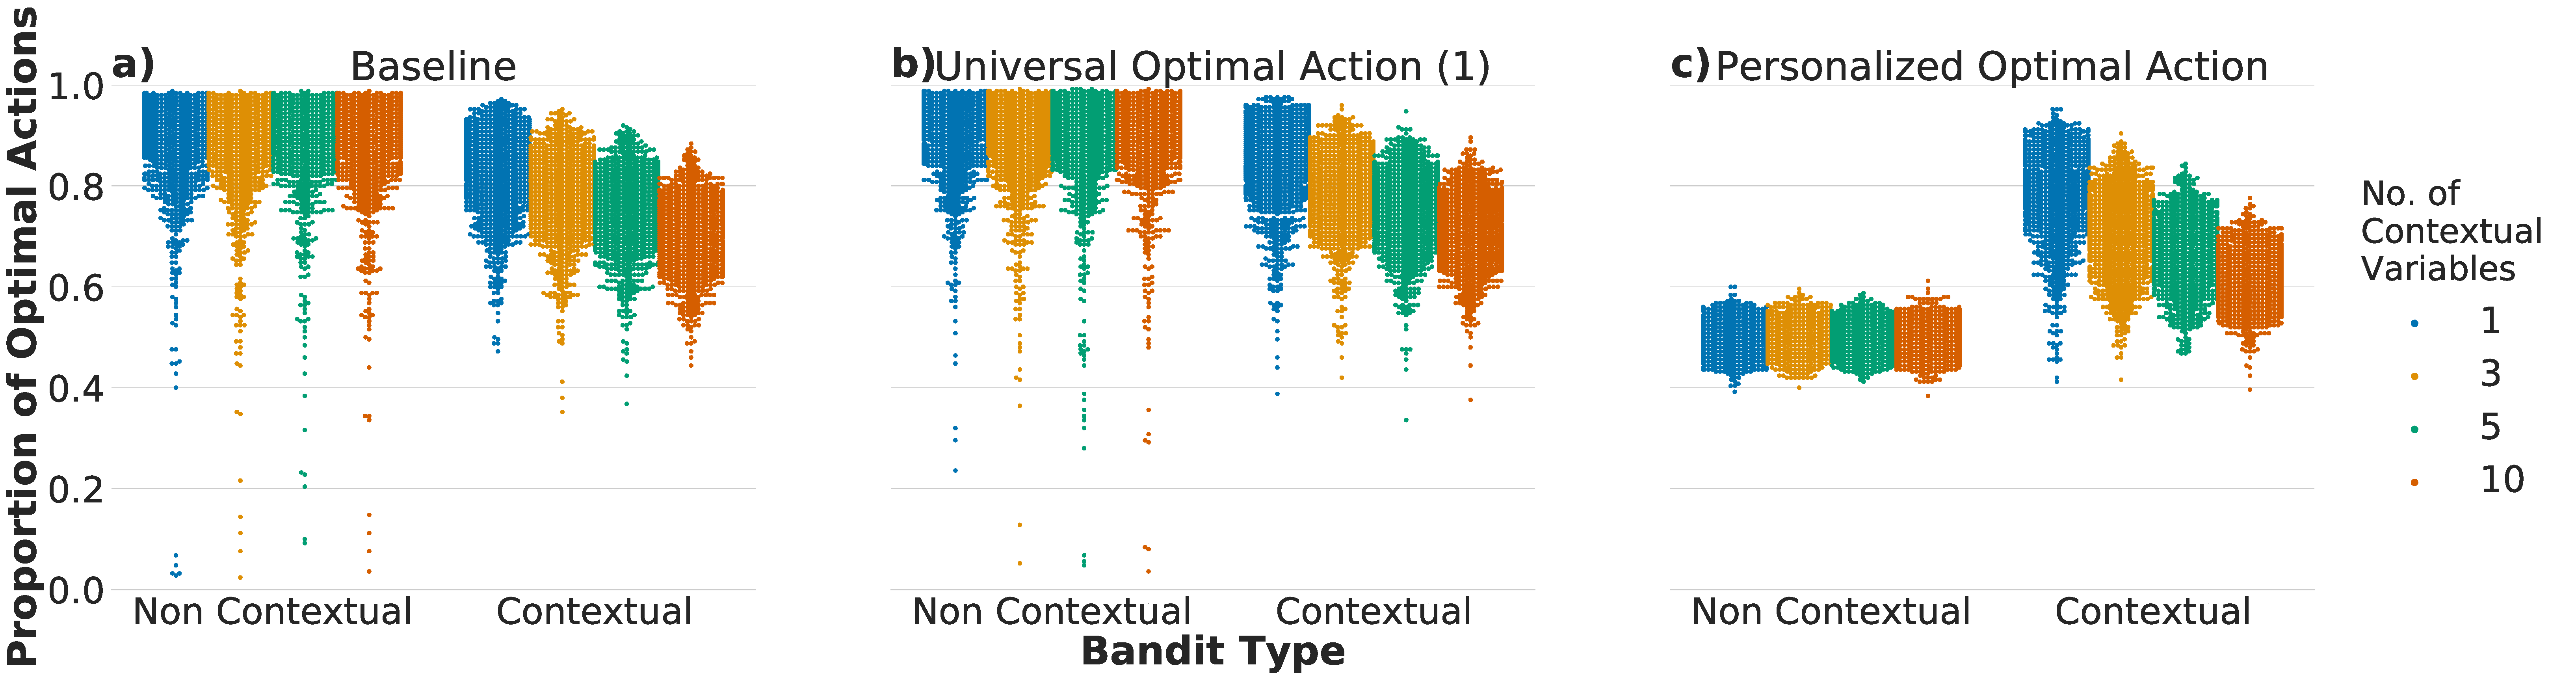
\includegraphics[width=\textwidth]{figs/NumConVars.pdf}
    \caption{Swarm plots for the proportion of optimal actions for the two bandit types. Each point represents results from one trial with 250 students. For the universal optimal action, all scenarios show similar results; hence only scenario (1) is shown. The decreased performance of the contextual bandits in the baseline and universal optimal action scenarios, especially for large number of contextual variables, highlights the potential risks of personalization.}
    \label{fig:NumConVars}
\end{figure*}

\begin{table*}[ht]
\begin{tabular*}{\textwidth}{@{\extracolsep{\fill}}llrlrlr}
\toprule
{} & Superior bandit &  $|b|$ &         95\% CI &  $F(1, 13996)$ &       $p$ &  Cohen's $d$ \\
\midrule
Baseline                     &  Non Contextual &  0.058 &  [0.052, 0.064] &       6308.000 &  $< .001$ &        1.279 \\
Universal Optimal Action (1) &  Non Contextual &  0.054 &   [0.048, 0.06] &       6333.000 &  $< .001$ &        1.278 \\
Universal Optimal Action (2) &  Non Contextual &  0.051 &  [0.048, 0.054] &      15762.000 &  $< .001$ &        1.892 \\
Universal Optimal Action (3) &  Non Contextual &  0.053 &   [0.047, 0.06] &       5918.000 &  $< .001$ &        1.240 \\
Universal Optimal Action (4) &  Non Contextual &  0.057 &  [0.049, 0.065] &       3180.000 &  $< .001$ &        0.927 \\
Personalized Optimal Action  &      Contextual &  0.272 &  [0.269, 0.276] &      34180.000 &  $< .001$ &        2.610 \\
\bottomrule
\end{tabular*}


\caption{Inferential statistics for proportion of optimal actions for the two bandit types across all outcome-generating models, simulated for 1000 trials of 250 students each. $b$ represents the coefficient of improvement of results for the superior bandit after controlling for the number of contextual variables.}
\label{table:resultsNumConVars}

\end{table*}

\begin{figure}[ht]
    \centering
    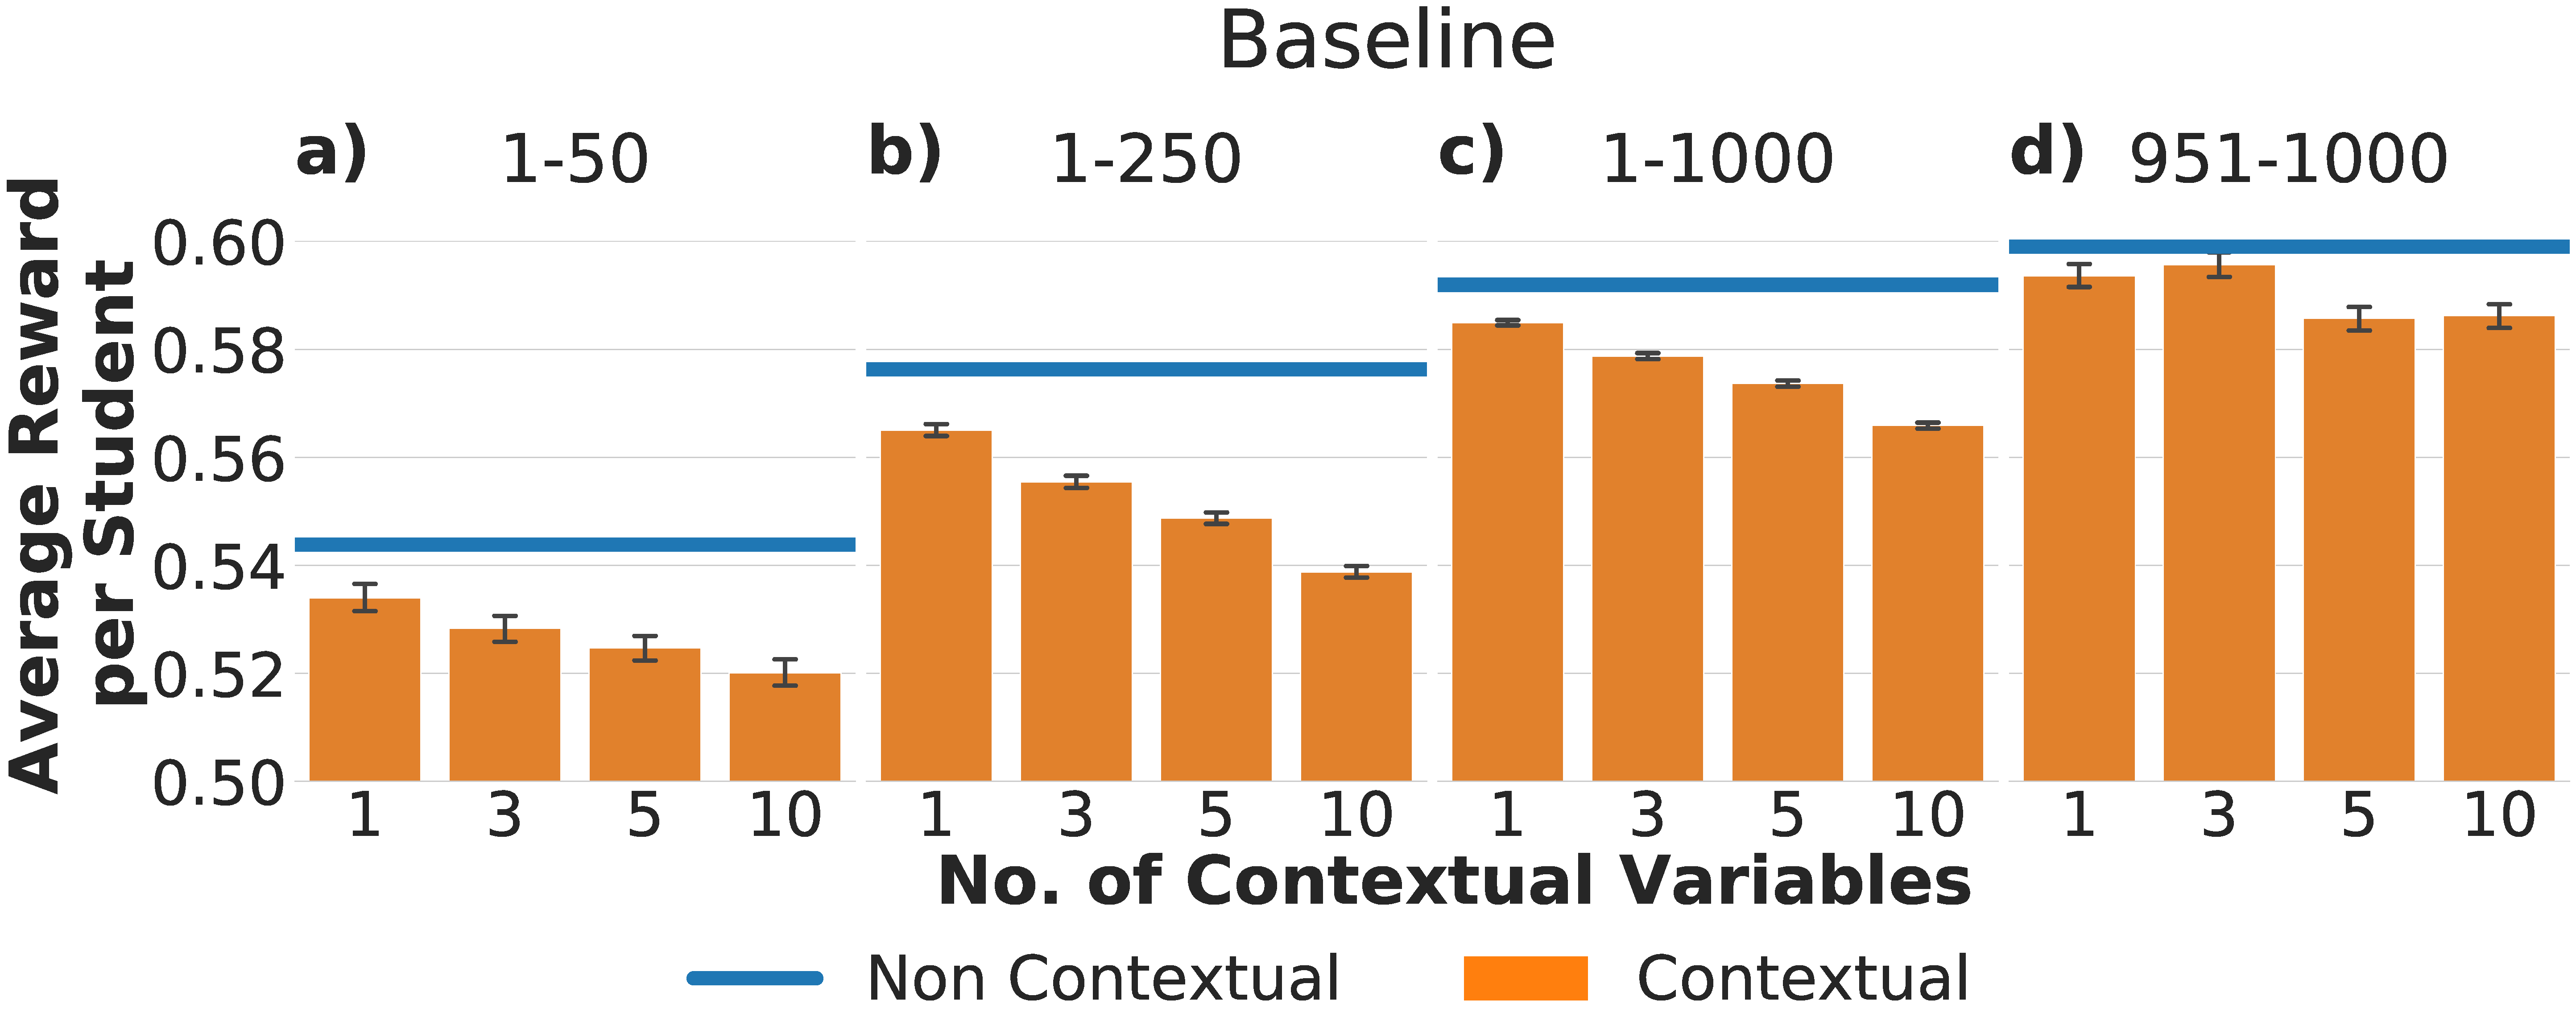
\includegraphics[width=\columnwidth]{figs/NumConVarsRanges.pdf}
    \caption{Average reward per student across 1--10 contextual variables for the two bandit types in the baseline model. In this model, the maximum possible expected reward is $0.6$, and the expected reward for uniform random assignment is $0.5$.
    % The bar graphs for the 4 time horizons are generated by simulating 1000-student classrooms over 1000 trials. 
    Error bars represent 1 standard error.}
    \label{fig:NumConVarsRanges}
\end{figure}

First we focused on analyzing the performance of contextual and non-contextual MAB algorithms for the three outcome-generating models across 1 to 10 student features (i.e., contextual variables).
Using an analysis of covariance (ANCOVA), we compared the two MAB algorithms' performance with respect to the proportion of optimal actions for 250 students across 1000 trials, treating the number of contextual variables as a covariate.
%An analysis of covariance (ANCOVA) were used to examine the difference in performance between the two bandit types, in terms of proportion of optimal actions for 250 students averaged over 1000 trials, while controlling for the number of contextual variables.

% The ANOVA model treats the proportion of optimal actions as the dependent variable, and the type of bandit and the number of contextual variables as a categorical and continuous dependent variables respectively

\textbf{Baseline:} When student features do not influence outcomes, we see that as expected, the non-contextual bandit outperforms the contextual bandit (Table~\ref{table:resultsNumConVars}): average performance per student for the final 50 out of 1000 students using the contextual algorithm is similar to that of the first 250 students using the non-contextual algorithm (Figure~\ref{fig:NumConVarsRanges}). 
As the number of student features increases, the contextual MAB chooses a lower proportion of optimal actions for the first 250 students (Figure~\ref{fig:NumConVars}a), but the effect is relatively small especially when considering the impact on actual reward ($t(13996)=-10.880$, $p<0.001$, $b=-0.006$, 95\% CI = $[-0.007, -0.005]$). At longer horizons, the number of student features has less of an impact on overall average reward (Figure~\ref{fig:NumConVarsRanges}), which we discuss more below.
% As shown in Figure~\ref{fig:NumConVarsRanges}, the impact of more student characteristics decreases as the number of students (horizon) increases: early on, more student characteristics necessitate more exploration, but after the algorithm has interacted with a large number of students (right,  Figure~\ref{fig:NumConVarsRanges}), that increased exploration early has resulted in higher rewards, as the extra exploration is likely to have resulted in more accurate estimates for how actions, student characteristics, and outcomes are related.


\textbf{Universal optimal action:} When outcomes are dependent on student features, the contextual MAB algorithm can learn a more accurate model than the non-contextual algorithm. However, when this more accurate model is not \textit{needed} for optimal action choices, learning the more accurate model does not improve action choices: the non-contextual bandit outperforms the contextual bandits in all four scenarios (Table~\ref{table:resultsNumConVars}; see Figure~\ref{fig:NumConVars}b for scenario 1).  While each scenario might arise due to different educational conditions, they are all very similar in how they appear to the non-contextual bandit algorithm.
The non-contextual bandit sees the two groups of students as identical, leading the overall performance to be the average for each group.
These changes in the average effectiveness of each intervention impact the algorithm's performance but do not necessarily degrade that performance; instead, the impact is dependent on how similar the two interventions are in their expected outcomes and how close those expected outcomes are to $0.5$, where there is the most variance.

\textbf{Personalized optimal action:} When the best policy for individual students depends on their features, the contextual bandit significantly outperforms the non-contextual bandit (Table~\ref{table:resultsNumConVars}). When only one student feature is included, the contextual MAB algorithm chooses the optimal action almost 70\% of the time for the first 50 students; this increases to almost 90\% for the final 50 of the total 250. Including extra student features decreases performance - if ten features are included and only one impacts the policy, the overall proportion of optimal actions falls to about 65\%. Yet, this is still an improvement over the non-contextual algorithm (Figure~\ref{fig:NumConVars}c).
These results suggest that even if a relatively small number of students will interact with the system and one is uncertain about which of a (limited) set of features will impact results, including those features will on average have a positive impact on student outcomes if one is confident that the best version of the system for an individual student varies based on one of those features.



\textbf{Variability across simulations:} Examining variability across simulations provides insight into how likely actual deployments of these algorithms are to reflect their average performance. Across all models, the contextual MAB algorithm exhibited greater variability in performance than the non-contextual MAB algorithm (Figure~\ref{fig:NumConVars}).
% more variability means that in many cases, the results may drift significantly from the averages, based on the variability in student responses. 
% While only the scenario involving a personalized optimal action resulted in better performance for the contextual MAB algorithm, variability of the contextual MAB algorithm's performance was consistently higher than the variability for the non-contextual MAB algorithm's performance. 
Surprisingly, increasing the number of student features leads to lower variance for the contextual MAB algorithm.  With small numbers of student features, there is often a concentration of simulations with lower achieved outcomes, resulting in bimodal distributions (Figure~\ref{fig:NumConVars}).   
The bimodality emerges because the algorithm can adapt more quickly, making it somewhat more vulnerable to underestimating parameter values based on a few samples with unexpected low rewards. Because the parameter estimates influence future action choices, data to correct these underestimates may not be collected quickly enough (as has been documented for non-contextual bandits in, e.g.,~\cite{erraqabi2017trading}). In contrast, increasing the number of student features increases variation near the mean but eliminates the bimodality (Figure~\ref{fig:NumConVars}) since the algorithm performs more exploration to learn the larger number of parameters. This makes it less likely to collect data that lead to erroneous conclusions about the effectiveness of actions. Errors in the parameter values are more likely to be corrected because they are unlikely to lead to the same choices for all student features, hence creating more variability in action choice for students with a specific value of a single feature. Indeed, the simulation results support these interpretations: for the baseline and universal optimal action models in a 1000-student classroom (see Figure~\ref{fig:NumConVarsRanges} for baseline), average reward for the first 250 students is lower but reward for the final 50 students is higher as the number of contextual variables increases.  There is thus a trade-off between expected outcomes and variability: the ability of the contextual MAB algorithm to adapt more quickly when it has fewer features to learn comes at the cost of it being less able to correct for wrong conclusions from small amounts of data.

% ANR: try to add something that explicitly calls out the horizon

% As shown in Table~\ref{table:stdev1Variable} [TODO: change to figure], the outcomes of the simulations using the contextual MAB algorithm are consistently more variable, regardless of the scenario, than the outcomes from the the non-contextual MAB algorithm. 
% \annanotes{would be nice to have the violin-type plots here for looking overall given just 1 variable and then looking at multiple variables just with the contextual and one of the three types of scenarios}

\textbf{Variability in policies across students}:
As noted above, the extra parameters learned by the contextual MAB algorithm lead to the potential for greater variability in action choices within a single simulation. This can systematically affect groups of students when the algorithm attaches spurious relevance to a feature that does not actually impact outcomes. We can see this pattern by examining differences in action probabilities for students who differ only by characteristics that do not impact outcomes: that is, considering all students who have the same value for the first feature, how does the probability of choosing a particular action change based on their different values for the other features?
As the number of contextual variables increases, the average maximum difference in action choice probability between such students also increases from 18--25\% when two student features are included in the model to over 90\% when ten features are included in the model after running through 250 students. This occurs both based on the greater expressivity of the model with more student features and the fact that the model with more student features is likely still learning about the impact of each of these features.
This raises potential concerns about inequity: students who should be treated identically by the system may instead be treated systematically differently, based on features that do not impact how they learn.


% \begin{itemize}
%     \item Want to add something here about in the average simulation with the non-contextual bandit, how different are the policies for students who are actually the same? Probably this gets done at a horizon endpoint, examining range and/or probability of assignment to each condition across students within group 1 as a whole and group 2 as a whole (for no effect, all students since groups don't matter).
% \end{itemize}


% \begin{table*}
% \caption{Proportion of optimal actions chosen by each MAB algorithm, based on the outcome-generating environment. The first three horizons correspond to average behavior across all students, given a fixed number of simulated students, while the final horizon is behavior at the end of the simulation, after the algorithm has learned from the first 950 student interactions. }
% \begin{tabular}{lrrrrr}
%                  &      \multicolumn{4}{}{Horizon}\\

% Quarter                 &      1-50 &      1-250 &              1-1000 &    951-1000 \\
% Bandit and Effect Type  &         &          &                   &                      \\
% ModContextual,None      & 0.69008 & 0.794872 &          0.846208 &              0.86748 \\
% ModContextual,Main (1)  & 0.70622 & 0.815184 &          0.867724 &              0.89082 \\
% ModContextual,Interaction48 &  0.75520 & 0.854288 &          0.893569 &     0.90876 \\
% ModContextual,Interaction57 &  0.69032 & 0.793884 &          0.845840 &     0.87096 \\
% ModContextual,Interaction89 &  0.66630 & 0.784140 &          0.845737 &     0.87476 \\
% ModContextual,Crossover & 0.68280 & 0.818588 &          0.890830 &              0.92334 \\
% NonContextual,None      & 0.73538 & 0.884636 &          0.959528 &              0.99170 \\
% NonContextual,Main (1)  & 0.74018 & 0.892628 &          0.962387 &              0.99172 \\
% NonContextual,Interaction48 &  0.80700 & 0.935956 &          0.979469 &     0.99674 \\
% NonContextual,Interaction57 &  0.73716 & 0.888996 &          0.960632 &     0.99154 \\
% NonContextual,Interaction89 &  0.70072 & 0.849556 &          0.941552 &     0.98550 \\
% NonContextual,Crossover & 0.50132 & 0.501544 &          0.500659 &              0.50000 \\

% \end{tabular}


% % \begin{tabular}{lrrrrr}
% % Quarter                 &      50 &      250 &              1000 &   201-250 &  951-1000 \\
% % Bandit and Effect Type  &         &          &                   &           &                    \\
% % ModContextual,Crossover & 0.68280 & 0.818588 &          0.890830 &   0.88412 &            0.92334 \\
% % ModContextual,Main      & 0.70622 & 0.815184 &          0.867724 &   0.86528 &            0.89082 \\
% % ModContextual,None      & 0.69008 & 0.794872 &          0.846208 &   0.84264 &            0.86748 \\
% % NonContextual,Crossover & 0.50132 & 0.501544 &          0.500659 &   0.50044 &            0.50000 \\
% % NonContextual,Main      & 0.74018 & 0.892628 &          0.962387 &   0.96374 &            0.99172 \\
% % NonContextual,None      & 0.73538 & 0.884636 &          0.959528 &   0.96042 &            0.99170 \\
% % \end{tabular}
% \end{table*}

% \begin{table*}[]
% \caption{Std dev TODO: improve caption, possibly combine with the other}\label{table:stdev1Variable}
% \begin{tabular}{lrrrrr}
% \toprule
% Quarter                 &        50 &      250 &             1000 &     201-250 &           951-1000 \\
% Bandit and Effect Type  &           &          &                   &             &                    \\
% ModContextual,Crossover &  0.212184 & 0.223219 &          0.207602 &    0.234230 &           0.210382 \\
% ModContextual,Main      &  0.216981 & 0.207370 &          0.204598 &    0.221534 &           0.208289 \\
% ModContextual,None      &  0.209366 & 0.218559 &          0.218536 &    0.238622 &           0.225952 \\
% NonContextual,Crossover &  0.072406 & 0.030994 &          0.015282 &    0.070336 &           0.071079 \\
% NonContextual,Main      &  0.199207 & 0.106869 &          0.046308 &    0.082158 &           0.034881 \\
% NonContextual,None      &  0.192135 & 0.104140 &          0.034901 &    0.067599 &           0.017246 \\
% \bottomrule
% \end{tabular}
% \end{table*}

% \annanotes{table we want here: proportion optimal action for contextual vs non-contextual at horizons of 0-50, 200-250, 0-250, 950-1000, 0-1000. Want this for all 5 scenarios. Idea is that gives us a sense of relatively short horizons (course with 50 students), medium horizon (course with 250 students, including difference in experience for initial and final students who interact with the system), and long horizon (course with 1000 students). Then also make this table for reward. For the group dependent reward scenarios, it would be nice to have another table that includes the same horizons but is just looking at the following alg/env: context, non-context, average of non-context with horizons halved and only one of the groups included (basically, removing the noise but retaining the mix of rewards - need to think about this one a little more, since it's sort of the separate contextual case...; maybe also compare to the same horizons but with one set of rewards or the other - that's asically an upper bound on how well we'd expect to do). Currently making that first table, although I think I'm likely missing a couple of the scenarios and will need to add them in. Need to run the simulations for the second non-contextual cases for that second table [this is currently happening].}


% \annanotes{
% To remake graphs in spring 2019 writeup:
% Summary_Statistics_PosterData_Clean_ModANR.ipynb : creates the data frame, including grabbing the appropriate students for each quarter (note that remaking the data frame takes a while)

% Bandit_Stats_Comparison_Graphing.ipynb: does the actual graphing based on the data frame created by the notebook above
% }
% \textbf{One contextual variable}\newline


% \vfill % Delete this to get rid of the column break!
\section{Impact of Uneven Distribution\\ of Student Characteristics} % This title needs to be improved... [snarky comment from ANR to herself]

\begin{figure}[t]
    \centering
    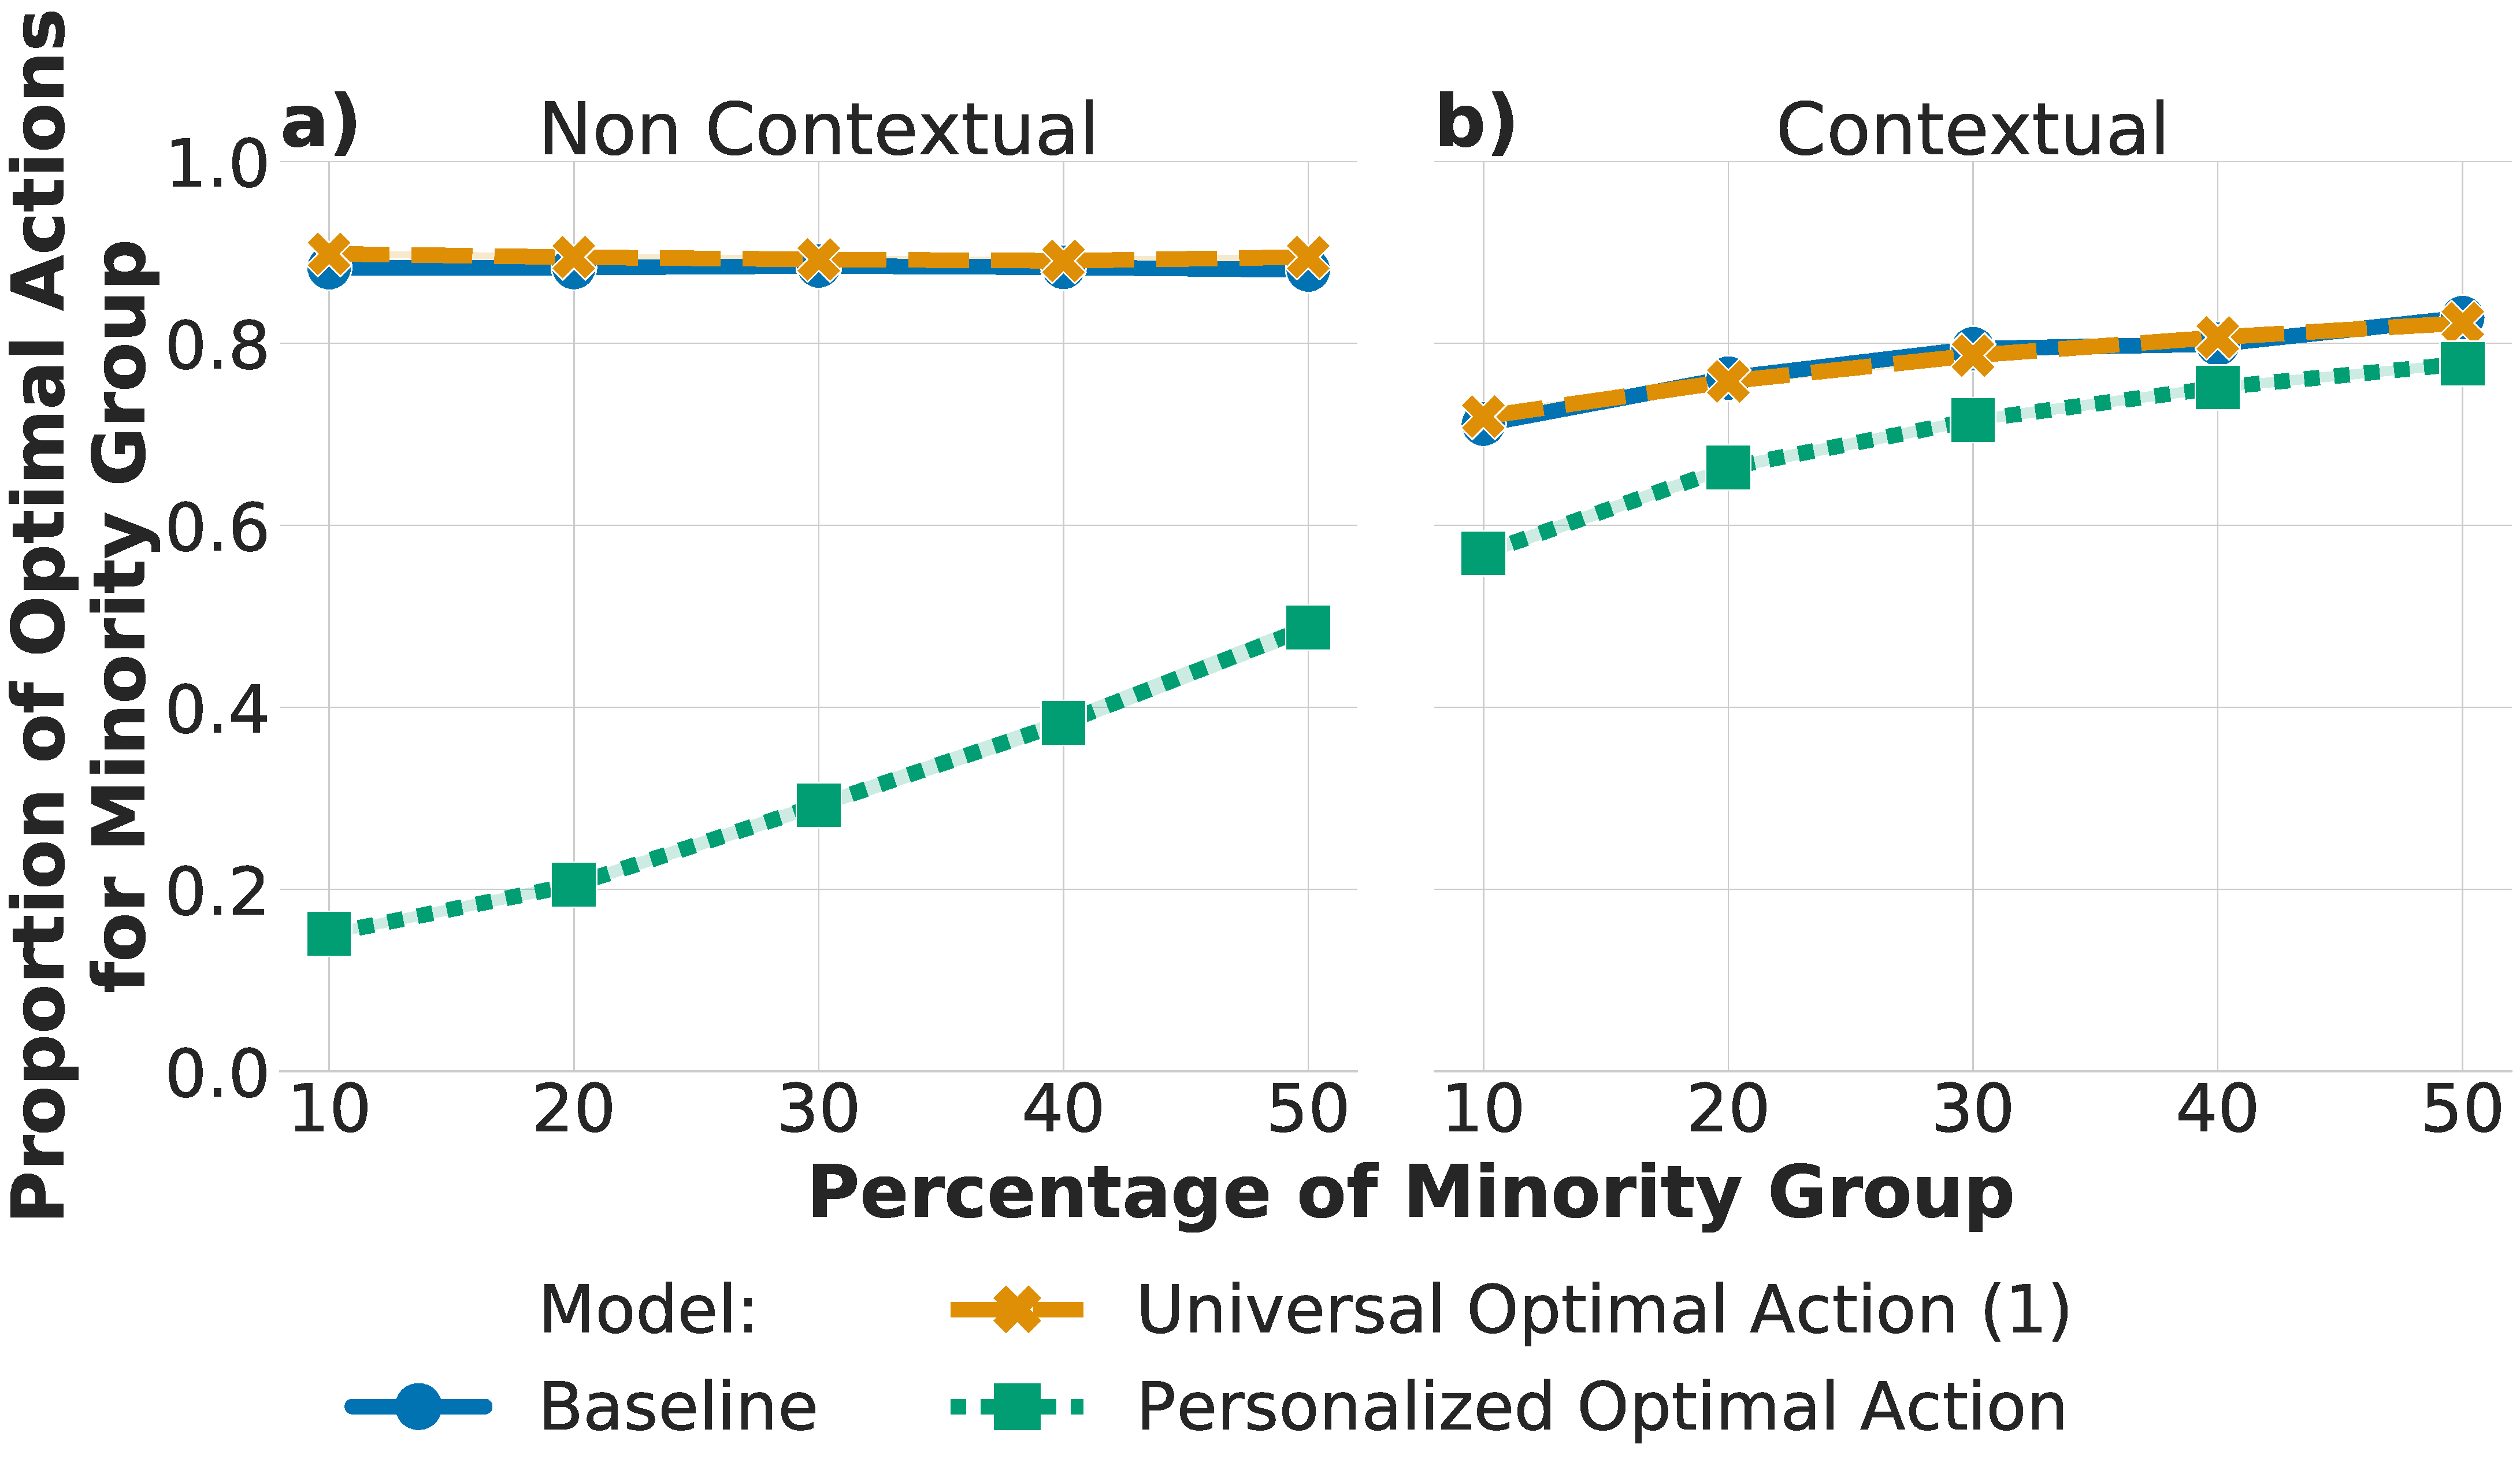
\includegraphics[width=\columnwidth]{figs/MinGrpSize.pdf}
    \caption{Proportion of optimal actions for minority groups with sizes of 10\%--50\% for the two bandit types across the three outcome-generating models, limited to one contextual variable. Standard errors, represented by the translucent bands, are negligible.}
    \label{fig:MinGrpSize1ConVar}
\end{figure}


The results of the previous simulations demonstrate that in situations where student characteristics (features) impact the outcome of different educational interventions, a contextual MAB algorithm only provides an improvement over a non-contextual algorithm when knowledge about the characteristic is necessary for choosing the best action. These simulations provided insight into how performance is impacted by different patterns of relationships between student characteristics and outcomes, with the assumption that those characteristics were uniformly distributed. However, in reality, some characteristics are likely to be more common than others. For example, when optimizing which hint to give to students who answer a question incorrectly, the algorithm is more likely to encounter a student with lower prior knowledge than one with higher prior knowledge.
% imagine a system that is choosing what intervention to give students who answer an exam question incorrectly. It is plausible that the most effective intervention is based on students' prior homework scores, but of students who answer incorrectly, more will tend to have low prior scores than high scores. 
Thus we now relax this assumption and explore how changing the distribution of student characteristics impacts student outcomes for both types of MAB algorithms. In these simulations, we examined not only overall outcomes, but also outcomes for different groups of students. Attention to group-specific outcomes is vital for identifying inequitable impacts of adaptive algorithms. %need to strengthen this point a bit


\subsection{Methods}

Similar to the first set of simulations, we compared non-contextual and contextual MAB implementations that used Thompson sampling across the same three horizons of 50, 250, and 1000 students, with a focus on 250; we repeated each simulation 1000 times. These simulations include a new independent variable: the proportion of students in each group. Specifically, for each simulated student, we varied the probability of the student being in the minority group (i.e., having a value of one for the first student characteristic) from 10\% to 50\%, using 10\% increments. 
% In our analyses of results, we group students into a minority group, which has the smaller probability of being enacted, and a majority group. At 50\%, the minority and majority groups have equal expected size.
In addition to analyzing performance across all students, we examined performance for both the minority and majority groups separately. We also examined the \textit{balanced success rate}, defined as the simple average of the group-specific performances~\cite{ben2010user}. Balanced success rate provides a way of examining performance that treats each group as equally important, even though one group may have more students than another.

\begin{figure*}[t]
    \centering
    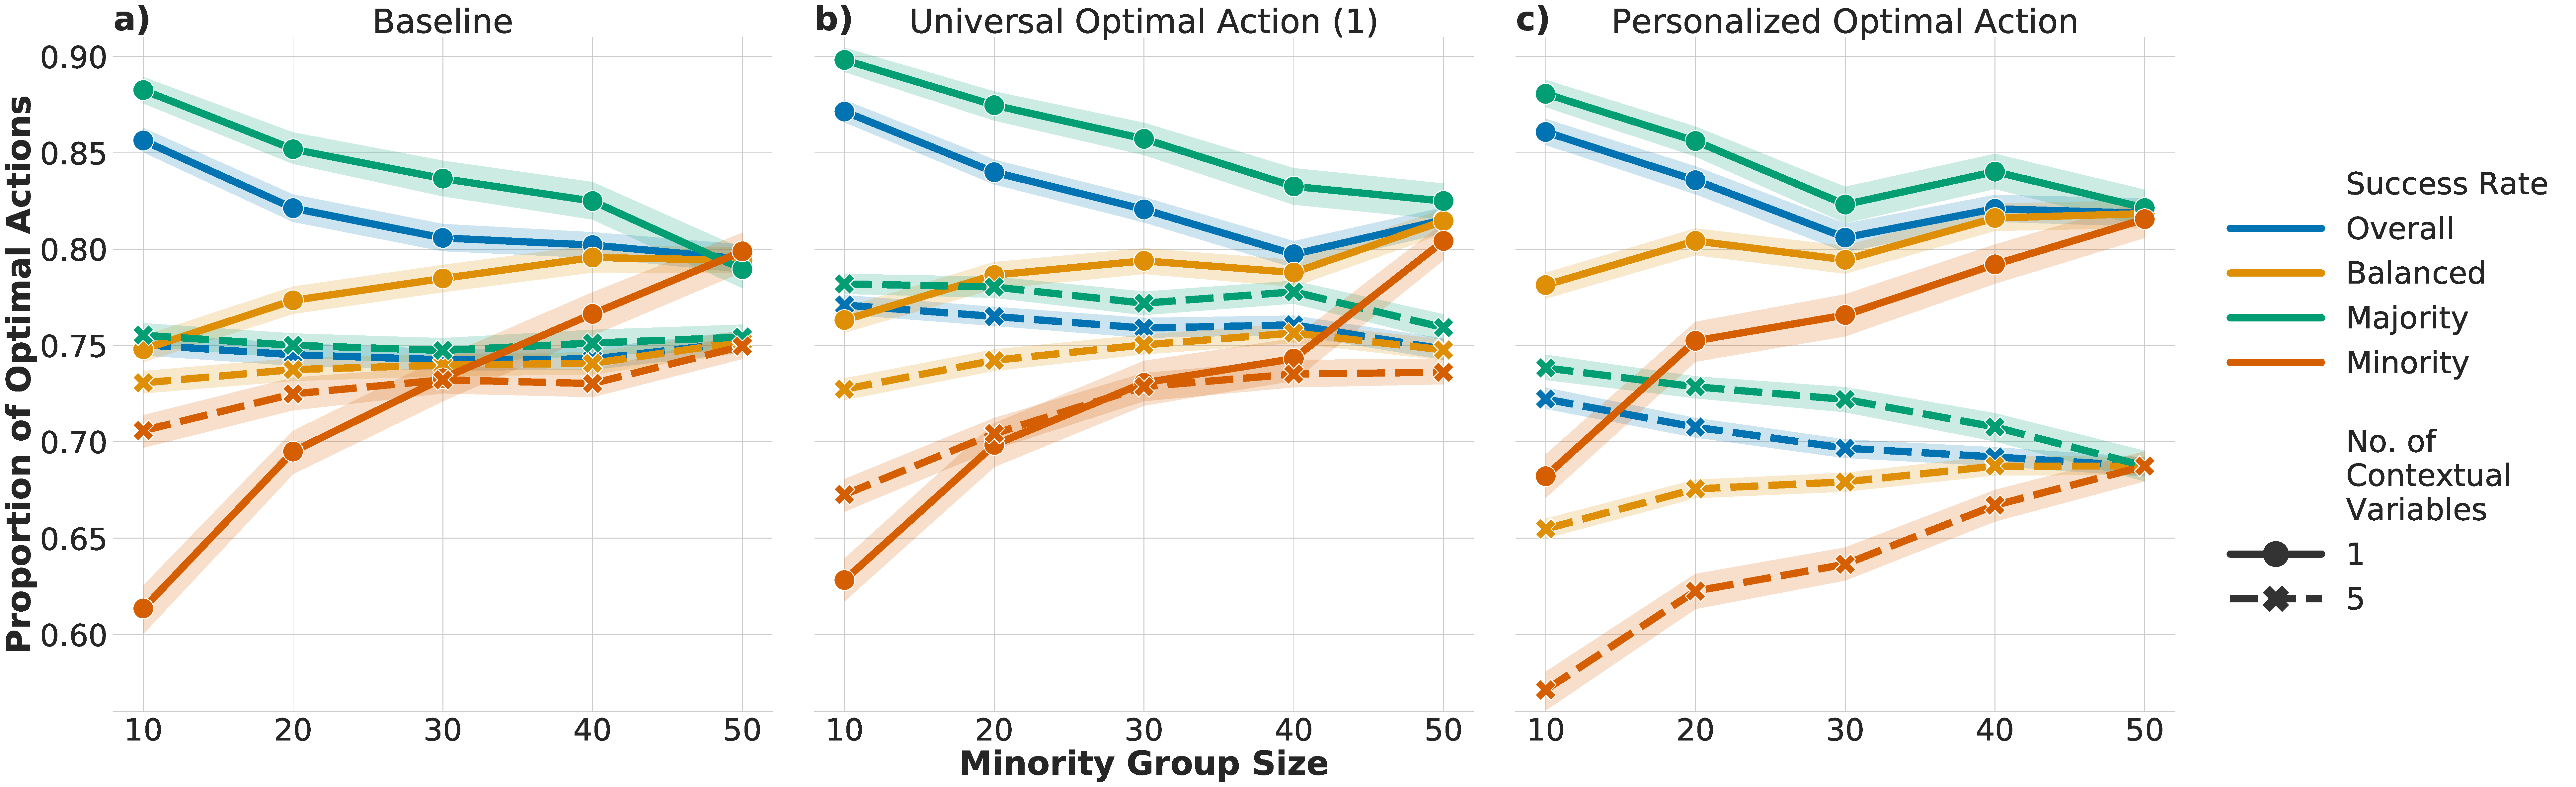
\includegraphics[width=\textwidth]{figs/MinGrpSize1v5.pdf}
    \caption{Comparing the proportion of optimal actions of the contextual bandit between 1 and 5 student features (i.e., contextual variables) for the majority and minority groups, as well as their balanced and overall averages, across minority group sizes of 10\%--50\%. Standard errors, represented by the translucent bands, are negligible.}
    \label{fig:Balanced_Success_Graph}
\end{figure*}
 
\subsection{Results}



% \begin{itemize}
%     \item First start with if we just have one contextual variable, what happens.
%     \item Then include something showing for one of the minority group sizes (20 or 30\%), what happens as the number of contextual variables increases.
%     \item Include some ANOVAs here to make sense of things.
% \end{itemize}


As in the previous analysis, we used an ANCOVA to compare the performance for the two bandit types in terms of the proportion of optimal actions, but this time treating the percentage of the minority group as a covariate. 

% Similar to the previous analysis, we focused on analyzing the performance of the two MAB algorithms for the three types of outcome-generating models for 250 students across 1000 trials. To compare the proportion of optimal actions across the two bandit types, we again used an ANCOVA, treating the percentage of the minority group as a covariate. 
%An analysis of covariance (ANCOVA) was used to examine the difference in performance between the two bandit types, in terms of proportion of optimal actions, while controlling for the percentage of the minority group.

\textbf{One student characteristic:} With one student characteristic, the contextual MAB algorithm's performance for the minority group decreases as the size of the minority group becomes smaller, across all outcome-generating models (Figure~\ref{fig:MinGrpSize1ConVar}b and Figure~\ref{fig:Balanced_Success_Graph}; $t(59996)=-33.962$, $p<0.001$, $b=-0.427$, 95\% CI = $[-0.452, -0.402]$).
This leads the contextual MAB algorithm to have a lower balanced success rate for smaller minority groups. However, overall performance across all students is slightly better since so many more students are in the majority group (Figure~\ref{fig:Balanced_Success_Graph}; $t(59996)=16.633$, $p<0.001$, $b=0.126$, 95\% CI = $[0.111, 0.141]$). In other words, decreasing the minority group size hurts the minority group more than it helps the majority group on a per-student basis; but replacing students from the minority group, who are assigned worse conditions, with students from the majority group, who are assigned better conditions, increases overall reward.  

This pattern of results occurs because the contextual MAB has more uncertainty about the impact of the particular value of the student characteristic that appeared fewer times: in the least balanced case, we expect the minority group to be seen only 25 times on average given a horizon of 250 students. Hence, providing a model with the potential to personalize for a minority group is a calculated risk - although the extra expressivity is likely intended to improve experiences for all groups of students, it can negatively impact minority groups, with a larger negative impact for smaller minority groups.

In contrast, the non-contextual MAB algorithm is relatively unaffected by the changing distribution of student characteristics in both the baseline ($t(9996)=0.497$, $p=0.619$) and universal optimal action scenarios ($t(39996)=1.506$, $p=0.132$), as shown by Figure~\ref{fig:MinGrpSize1ConVar}a. The changing distribution of student characteristics changes the expected rate of obtained reward from each action, but the changes are small enough that they have little impact on the algorithm's ability to choose optimal actions.
% This is perhaps surprising in the latter case because as the distribution of students changes, the amount of variance in each condition is also changed. For example, in one of the four group independent policy cases, a student in the minority group has a positive outcome 80\% of the time with action 1 and 90\% of the time with action 2, compared to 40\% and 60\% for a student in the majority group. There is a slight trend in this case for lowered performance given a moderate amount of students in the minority group, with the poorest performance occurring with 30\% of students in the minority group, but the overall difference in performance is slight. 

However, for the personalized optimal action model, the size of the minority group \textit{does} have a large impact on individual student outcomes for the non-contextual MAB algorithm: when the minority group is small, the algorithm learns to choose the action that is best for the majority and worst for the minority, resulting in the optimal action being chosen only 15\% of the time for the minority group, within a horizon of 250 students (Figure~\ref{fig:MinGrpSize1ConVar}a). When the two groups are of equal size, the algorithm has no systematic information that shows one action as consistently better or worse than the other; thus on average, it chooses the optimal action about 50\% of the time for both groups. 


\textbf{Additional student characteristics for the contextual MAB algorithm:} When the number of student characteristics increases, the impact on the minority and majority groups differs for the baseline and universal optimal action models compared to the personalized optimal action  (Figure~\ref{fig:Balanced_Success_Graph}). In the two former models, the impact on balanced success rate is generally small: as the number of student characteristics increases from one to five, balanced success decreases no more than 8\%, except by 11\% in universal optimal action (4); for most of these models, the decrease is even smaller when the minority group is smaller.
In these models, the algorithm's performance for small minority groups is improved with more student characteristics, while performance for majority groups decreases. For example, in the baseline scenario with 10\% of students in the minority group, the algorithm chooses the optimal action for 71\% of the minority group when there are five student characteristics, compared to 61\% of these students when there is only one student characteristic.
More student characteristics leads to more exploration with the initial students, and thus the algorithm is less likely to systematically execute a bad policy for the minority group based on a small number of initial samples. 

% balanced success rate for the contextual MAB algorithm decreases, regardless of the size of the minority group or outcome-generating scenario.
% The pattern of results that generates this lowered success rate 
% Increasing the number of contextual variables tends to hurt the majority group, while helping the mino
% However, the difference in balanced success rates is largest when the two groups are of equal size, and with the exception of the personalized optimal action scenario, the difference in balanced success rates tends to be smaller when the minority group is smaller. 
% This results from the fact that, again with the exception of the personalized optimal action scenario, the algorithm's performance for small minority groups is actually better with more contextual variables. For example, in the baseline scenario with 10\% of students in the minority group, the algorithm chooses the optimal action for 71\% of the 250 students when there are five contextual variables, compared to 61\% of the students when there is only one contextual variable. This occurs because more contextual variables leads to more exploration with the initial students, and thus the algorithm is less likely to systematically execute a suboptimal policy for the minority group due to drawing conclusions from a small number of initial samples. 

For the personalized optimal action scenario, increasing the number of student characteristics from one to five decreases performance for both minority and majority groups by about 15\% regardless of the size of the minority group, uniformly lowering balanced success rate. Due to the extra exploration caused by the extraneous student characteristics, the algorithm is slower to exploit the actual relationship between the relevant student characteristic and the action choice, without differential impact based on minority group size.
%, combined with fewer students from which to learn about the minority group, means that the extra exploration that improves performance in the other scenarios hurts performance in this case: the algorithm is less quick to exploit the actual relationship between the relevant student characteristic and the action choice.

% Key patterns:
% \begin{itemize}
%     \item When minority group is small, there's improved performance *for the minority group* with 5 variables for most scenarios. Reason: more exploration early on, less likely to systematically fall into a suboptimal policy for any particular group.
%     \item But as minority group size grows, performance changes less quickly with 5 CVs: more exploration still happening at the same horizon, because less confident in conclusions.
%     \item For the case where the policy does depend on the CV, there's decreased performance for the minority group for all of the minority group sizes when there are 5 CVs. That's because the extra CVs make it harder to find a true interaction when there is one.
%     \item BSR: Lower for CV = 5 as expected. Appears that as minority group size increases, for all but crossover the difference in performance increases slightly. For crossover, size of effect is relatively constant.
% \end{itemize}

\iffalse % block comment


\begin{table*}
\caption{Proportion optimal actions, horizon = 250, all group sizes, performance across all groups and CV = 1.}
\begin{tabular}{lrrrrr}
\toprule
Minority Group Size &        10 &        20 &        30 &        40 &        50 \\
Bandit and Effect Type      &           &           &           &           &           \\
\midrule
ModContextual,None      &  0.856348 &  0.821244 &  0.805808 &  0.802108 &  0.794872 \\
ModContextual,Main (1)      &  0.871400 &  0.839916 &  0.820596 &  0.797332 &  0.815184 \\
ModContextual,Interaction48 &  0.933624 &  0.907804 &  0.887108 &  0.866224 &  0.854288 \\
ModContextual,Interaction57 &  0.855780 &  0.820044 &  0.804564 &  0.804548 &  0.793884 \\
ModContextual,Interaction89 &  0.790200 &  0.790876 &  0.764876 &  0.781476 &  0.784140 \\
ModContextual,Crossover &  0.860764 &  0.835756 &  0.805980 &  0.820940 &  0.818588 \\
NonContextual,None      &  0.891668 &  0.877504 &  0.883992 &  0.883216 &  0.884636 \\
NonContextual,Main (1)      &  0.899700 &  0.899288 &  0.897256 &  0.884064 &  0.892628 \\
NonContextual,Interaction48 &  0.959292 &  0.957744 &  0.949364 &  0.944288 &  0.935956 \\
NonContextual,Interaction57 &  0.890644 &  0.883288 &  0.890980 &  0.887544 &  0.888996 \\
NonContextual,Interaction89 &  0.838168 &  0.826292 &  0.823028 &  0.841332 &  0.849556 \\
NonContextual,Crossover &  0.776756 &  0.670608 &  0.580048 &  0.521512 &  0.501544 \\
\bottomrule
\end{tabular}
\end{table*}

\begin{table*}
\caption{Proportion optimal actions, horizon = 250, all group sizes, performance for group 0 and CV = 1.}
\begin{tabular}{lrrrrr}
\toprule
Minority Group Size &        10 &        20 &        30 &        40 &        50 \\
Bandit and Effect Type      &           &           &           &           &           \\
\midrule
ModContextual,None      &  0.613523 &  0.694961 &  0.732960 &  0.766390 &  0.798822 \\
ModContextual,Main (1)     &  0.628272 &  0.698429 &  0.730649 &  0.743170 &  0.804242 \\
ModContextual,Interaction48 &  0.595183 &  0.702625 &  0.730411 &  0.750989 &  0.782653 \\
ModContextual,Interaction57 &  0.622903 &  0.678792 &  0.717704 &  0.779673 &  0.796462 \\
ModContextual,Interaction89 &  0.598684 &  0.678936 &  0.743387 &  0.774596 &  0.823764 \\
ModContextual,Crossover &  0.682151 &  0.752437 &  0.765803 &  0.792061 &  0.815562 \\
NonContextual,None      &  0.893786 &  0.876132 &  0.883945 &  0.884595 &  0.883612 \\
NonContextual,Main (1)     &  0.901123 &  0.898164 &  0.898399 &  0.883778 &  0.892063 \\
NonContextual,Interaction48 &  0.958717 &  0.957539 &  0.949884 &  0.944494 &  0.936221 \\
NonContextual,Interaction57 &  0.891941 &  0.884045 &  0.890403 &  0.887577 &  0.890546 \\
NonContextual,Interaction89 &  0.836723 &  0.828386 &  0.823892 &  0.841261 &  0.849212 \\
NonContextual,Crossover &  0.149687 &  0.213161 &  0.294141 &  0.379826 &  0.484818 \\
\bottomrule
\end{tabular}
\end{table*}

\begin{table*}
\caption{Balanced success rate for proportion optimal actions - horizon = 250, 1 CV}
\begin{tabular}{lrrrrr}					
\toprule					
Minority Group Size &        10 &        20 &        30 &        40 &        50 \\					
Bandit and Effect Type - BSR  &           &           &           &           &           \\					
\midrule					
ModContextual,None      	   &    0.748016	& 0.773401	& 0.7847735	& 0.795648	& 0.794208      \\
ModContextual,Main      	   &    0.7632115	& 0.7865455	& 0.793931	& 0.78784	  & 0.8145985     \\
ModContextual,Interaction48  &    0.7831475	& 0.8307925	& 0.842807	& 0.8463	  & 0.8539765     \\
ModContextual,Interaction57  &    0.7521865	& 0.7665245	& 0.7793055	& 0.79957	  & 0.793037      \\
ModContextual,Interaction89  &    0.7045975	& 0.748741	& 0.7585305	& 0.779965	& 0.783931      \\
ModContextual,Crossover 	   &    0.7813535	& 0.8042625	& 0.794461	& 0.8161455	& 0.8184485     \\
NonContextual,None      	   &    0.8926215	& 0.8769845	& 0.883969	& 0.8834765	& 0.884669      \\
NonContextual,Main      	   &    0.900343	& 0.898902	& 0.897586	& 0.884048	& 0.892659      \\
NonContextual,Interaction48  &    0.959022	& 0.957682	& 0.9494705	& 0.944336	& 0.9359175     \\
NonContextual,Interaction57  &    0.891247	& 0.883549	& 0.8908255	& 0.8875825	& 0.88897       \\
NonContextual,Interaction89  &    0.837544	& 0.8271395	& 0.8232795	& 0.8413645	& 0.849524      \\
NonContextual,Crossover 	   &    0.49779 	& 0.4982355	& 0.497484	& 0.496847	& 0.4987915     \\
\bottomrule					
\end{tabular}
\end{table*}

\begin{table*}
\caption{Proportion optimal actions, horizon = 250, all group sizes, performance for group 1 and CV = 1.}

\begin{tabular}{lrrrrr}
\toprule
Minority Group Size &        10 &        20 &        30 &        40 &        50 \\
Bandit and Effect Type  &           &           &           &           &           \\
\midrule
ModContextual,None      &  0.882509 &  0.851841 &  0.836587 &  0.824906 &  0.789594 \\
ModContextual,Main      &  0.898151 &  0.874662 &  0.857213 &  0.832510 &  0.824955 \\
ModContextual,Interaction48 &  0.971112 &  0.958960 &  0.955203 &  0.941611 &  0.925300 \\
ModContextual,Interaction57 &  0.881470 &  0.854257 &  0.840907 &  0.819467 &  0.789612 \\
ModContextual,Interaction89 &  0.810511 &  0.818546 &  0.773674 &  0.785334 &  0.744098 \\
ModContextual,Crossover &  0.880556 &  0.856088 &  0.823119 &  0.840230 &  0.821335 \\
NonContextual,None      &  0.891457 &  0.877837 &  0.883993 &  0.882358 &  0.885726 \\
NonContextual,Main      &  0.899563 &  0.899640 &  0.896773 &  0.884318 &  0.893255 \\
NonContextual,Interaction48 &  0.959327 &  0.957825 &  0.949057 &  0.944178 &  0.935614 \\
NonContextual,Interaction57 &  0.890553 &  0.883053 &  0.891248 &  0.887588 &  0.887394 \\
NonContextual,Interaction89 &  0.838365 &  0.825893 &  0.822667 &  0.841468 &  0.849836 \\
NonContextual,Crossover &  0.845893 &  0.783310 &  0.700827 &  0.613868 &  0.512765 \\
\bottomrule
\end{tabular}
\end{table*}

\fi


\section{Real-World Experiments}

\begin{table*}[t]
\label{table:realworldSimSetups}
\centering
\begin{tabular*}{\textwidth}{lr@{\extracolsep{\fill}}rllll}
    \toprule
                                & Problem Set & Students & Q1 Size      & Q2 Size      & Q3 Size     & Q4 Size     \\
    \midrule
    Uneven Student Distribution & 293151      & 320      & 113 (35.3\%) & 100 (31.3\%) & 69 (21.6\%) & 38 (11.9\%) \\
    Even Student Distribution   & 263057      & 129      & 33 (25.6\%)  & 28  (21.7\%) & 34 (26.4\%) & 34 (26.4\%) \\
    \bottomrule
\end{tabular*}
\caption{Student totals and group distributions in the original ASSISTments data \cite{selent2016assistments} for the two problem sets of interest. Prior percent correct is discretized before removing students who have never answered incorrectly to experience the assigned condition, biasing group size towards the lower quartiles in the Uneven Student Distribution.}
\end{table*}

\begin{figure*}[t]
    \centering
    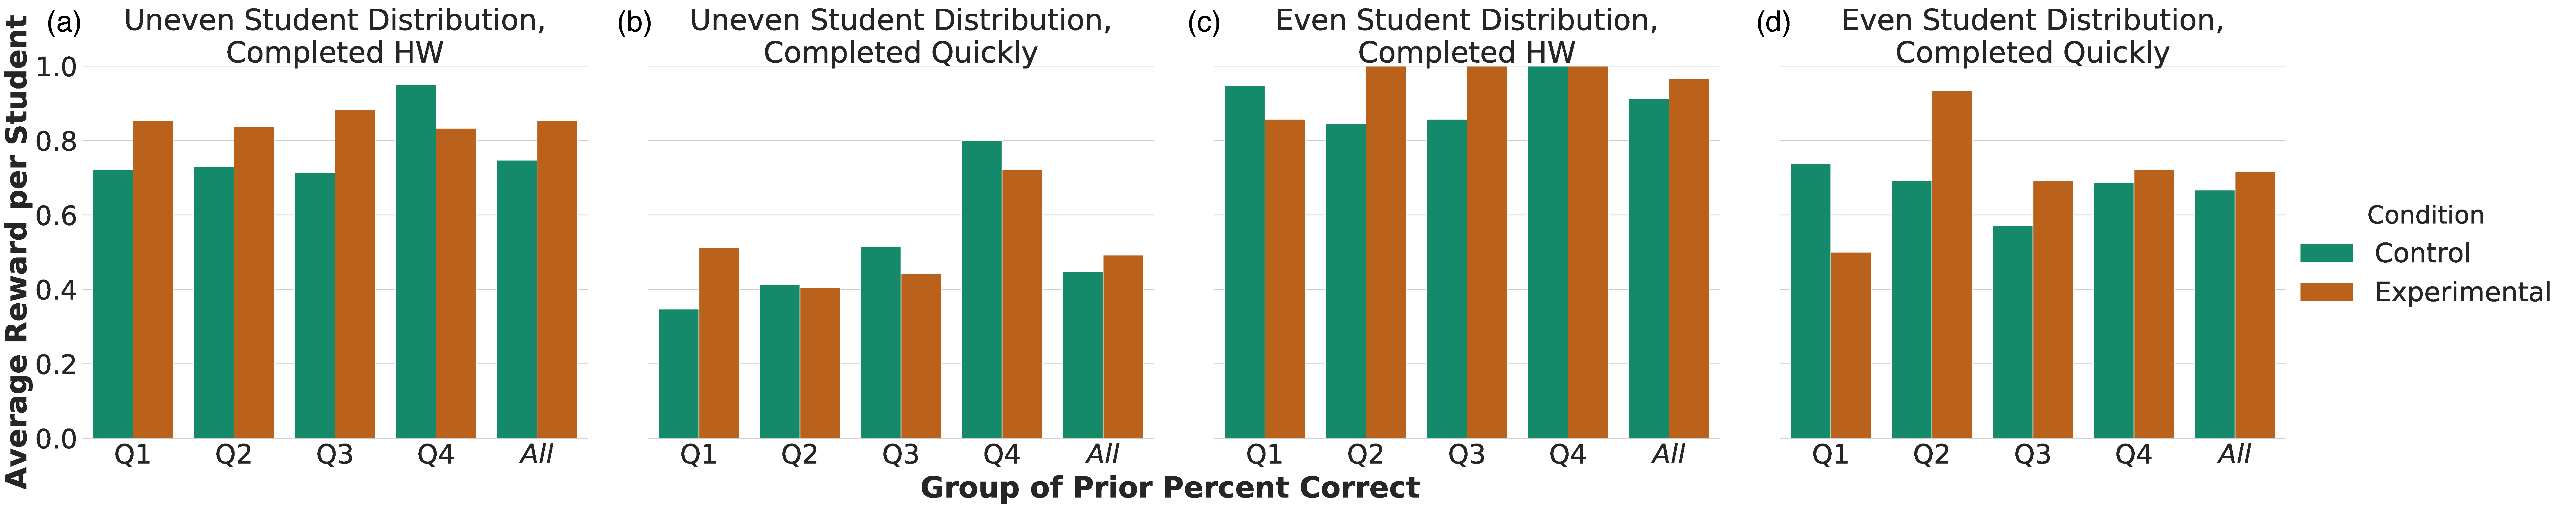
\includegraphics[width=\textwidth]{figs/RealWorld_OriginalProbsLabeled.pdf}
    \caption{Original average reward per student in the ASSISTments data \cite{selent2016assistments}, across the four quartiles (Q1--Q4) of prior percent correct and their averages, for the two conditions in the experiments (control and experimental) illustrates our model parameters of real-world scenarios.}
    %The bar graphs for the four simulation scenarios (two problem sets x two outcome measures) show average rewards across the four quartiles (Q1--Q4) and overall of prior percent correct.}
    % \caption{Average reward per student, calculated from the original ASSISTments data \cite{selent2016assistments} to show the real-world parameters, for the two conditions in the experiment (control and experimental). The bar graphs for the four simulation scenarios (two problem sets by two outcome measures) show mean reward across the four quartiles of prior percent correct (Q1--Q4) and overall.}
    \label{fig:realworldParameters}
\end{figure*}

The first two sets of simulations can guide system designers when making decisions about personalizing based on student features. However, they have some limitations: while they considered a relatively large space of possibilities for how outcomes relate to student features, they focused on showing a general variety of cases rather than on specific cases that might be most common or of particular interest in education. To address this, we conducted several case studies of how MAB algorithms would have impacted actual experiments. We consider existing experimental data in which the optimal action would be personalized to see if the contextual MAB algorithms benefits students (as would be expected from our previous simulations) and also to demonstrate how factors from the previous simulations manifest in real-world scenarios. 

The experiments were previously conducted within \textit{ASSISTments}, an online learning system, and focused primarily on middle school math. We selected several experiments from~\cite{selent2016assistments}  based on how student outcomes were related to their prior successes in the system as well as their assignment of either the control or experimental condition. Prior success in the system is a strong candidate to be a student feature for personalization: it is typically easily available and can serve as a proxy for prior knowledge, which has been shown to influence the success of different instructional strategies~\cite{shute2008focus}. 
% that we focus on were all conducted as randomized controlled trials within ASSISTments. ASSISTments is an online math learning system to teach math to students in grades 4-12 within the United States. The experiments that we focused on mainly involved middle school math students in Massachusetts. We chose several of the 22 experiments presented in previous work~\cite{selent2016assistments} based on how student outcomes were related to their prior success in the system as well as their condition assignment. Prior success in the system is a strong candidate for the type of student characteristic that designers might want to use for personalization because it can serve as a proxy for prior knowledge that is typically easily available in a system and a number of past studies have shown that prior knowledge can influence the success of different instructional strategies. 

\subsection{Methods}

To model previously collected ASSISTments data in our MAB framework, we (1) transformed both the student characteristics and the student outcomes into discrete variables,\footnote{MAB algorithms can handle non-categorical data, but we focus on the categorical case to mirror our prior simulations.} and (2) resampled from the data to generate outcomes when the MAB algorithm assigned a condition.


For step (1), we first discretized students' prior percent correct on problems within ASSISTments, the sole student feature that we included for personalization, into four quartiles: the 25\% of students who began the homework assignment with the lowest prior percent correct (Q1), then those in the 26--50\% range (Q2), and so on. The dataset contains some students who began the homework but were not assigned to a condition. Since the experiments in~\cite{selent2016assistments} mainly manipulated students' experiences (e.g. type of hint) when they answered a question incorrectly, students who have never answered incorrectly are not included in the experiment results (nor will the MAB algorithm make choices for them). However, they are included in the quartile cutoffs, which means that in the population of students with whom the MAB algorithm interacts, the number of students in each quartile may not be uniform.
% re are not necessarily an equal number of students in each quartile. Some of our simulations thus touch on the case where student characteristics are unevenly distributed.

We also chose and discretized the student outcome measures. These experiments included two different measures of student outcomes: whether each student completed the homework and the number of problems that each student answered in the homework. 
All experiments took place in the \textit{SkillBuilder} interface, where students must answer three consecutive problems correctly to complete the homework. 
Completion of homework (denoted \textit{Completed HW}) is already discrete and could easily be collected in real time; two of our simulations use this measure. 
However, it is relatively coarse, as the vast majority of students completed the homework.
% : most students do complete the homework, and they may do so even if the hints or explanations they're receiving are relatively ineffective due to external motivations. 
Thus, we also used a discretized version of the number of problems to completion (denoted \textit{Completed Quickly}). If a student completes the homework, doing so in fewer problems is a better outcome than doing so in more problems. Outcomes were based on the median problem count for students who completed the homework. Students who completed the homework in the median number of problems or fewer had positive reward, while those who did not complete the homework or completed it more slowly had no reward.
% Specifically, students who did not complete the homework were assigned no reward under this outcome measure. Then, the median of the problem count for the remaining students was used to divide their reward in a binary manner: students who completed the task in the median number of problems or below received a reward; students who took more than the median number of problems to complete did not. 
Though for practical use prior data would be needed to select an appropriate cut point, using a cut point based on collected data in our simulations measures the performance of students more closely.

% We used two types of models to evaluate MAB performance on these data, following the procedure of Rafferty, Ying and Williams (2019): parameter models and outcome models. The parameter models fit a logistic regression to the observed reward by the contextual variables of the students. Using the learned intercepts for each action and coefficients for each encoded contextual variable, the model would then run trials in the same manner as outlined in the previous methods section, using the real group proportions. Each trial in a parameter model would thus represent a classroom with similar composition and performance characteristics to the classroom from the original experiment.



% Like other recent work examining MAB behavior through simulation of experimental studies~\cite{rafferty2019statistical}, we 
% The outcome models were designed to model the classroom more directly by drawing from the observed contextual vectors and rewards. Specifically, for each of the trials, the students' context vectors were drawn in a random order, and observed rewards for each combination of action and context vectors were likewise sampled in random order. These orders remained consistent between the contextual and non-contextual MAB within a given trial, such that each trial in an outcome model would represent a classroom of students drawn with replacement from the students from the original experiment.







% \begin{figure*}[t]
%     \centering
%     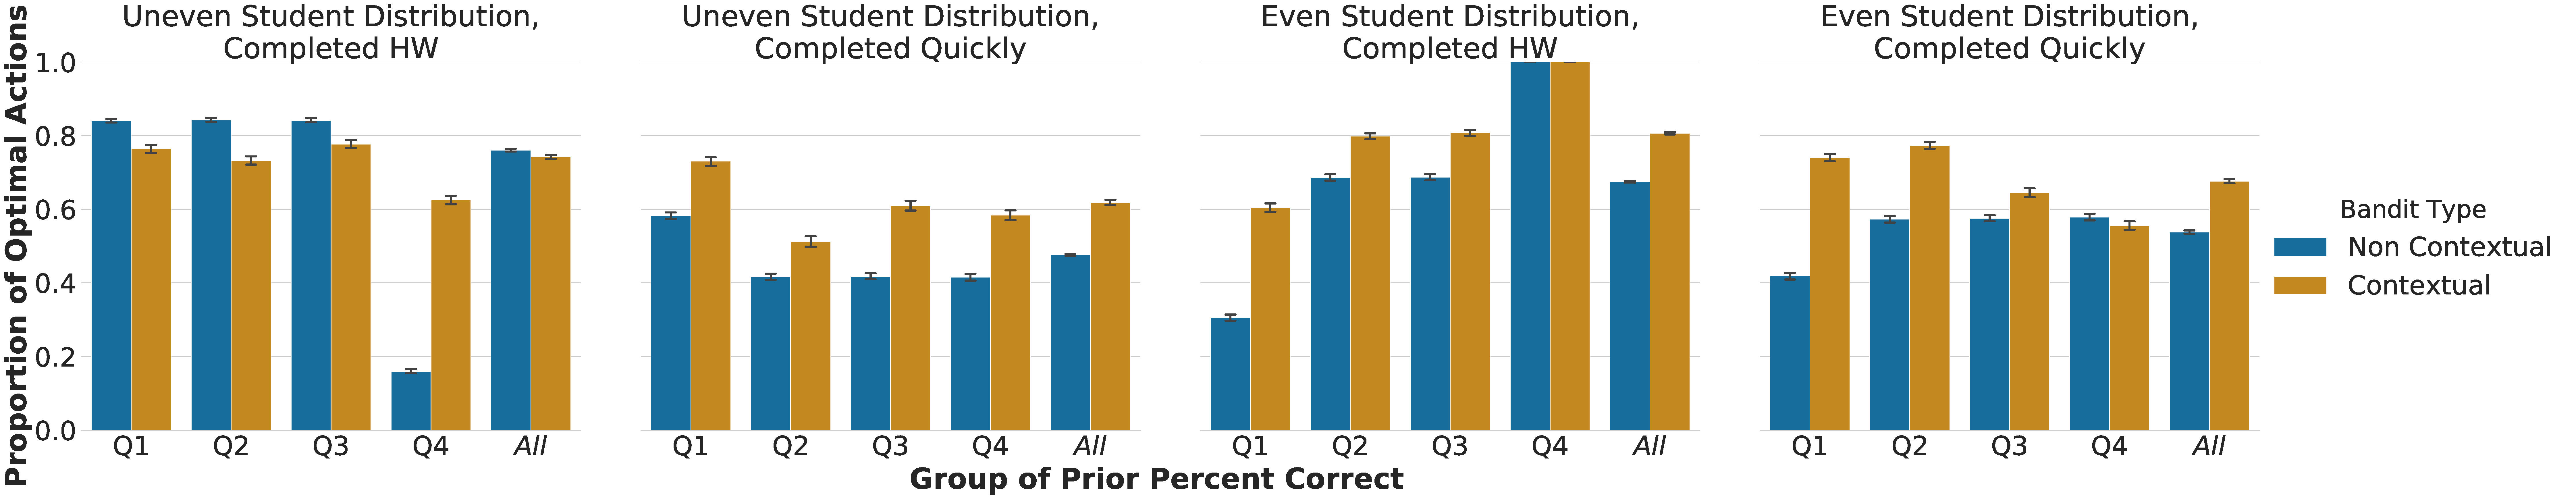
\includegraphics[width=\textwidth]{figs/RealWorld_PropOptimal.pdf}
%     \caption{Proportion of optimal actions across the four quartiles of prior percent correct (Q1--Q4) and overall for the two bandit types. 
%     %The bar graphs for the four simulation scenarios are generated by simulating classrooms with their original number of students over 1000 trials. 
%     Error bars represent 1 standard error. The extra information learned by the contextual bandit enables it to improve optimal action choice rate in most cases.}
%     \label{fig:realworldOptimal}
% \end{figure*}



% \begin{figure*}
%     \centering
%     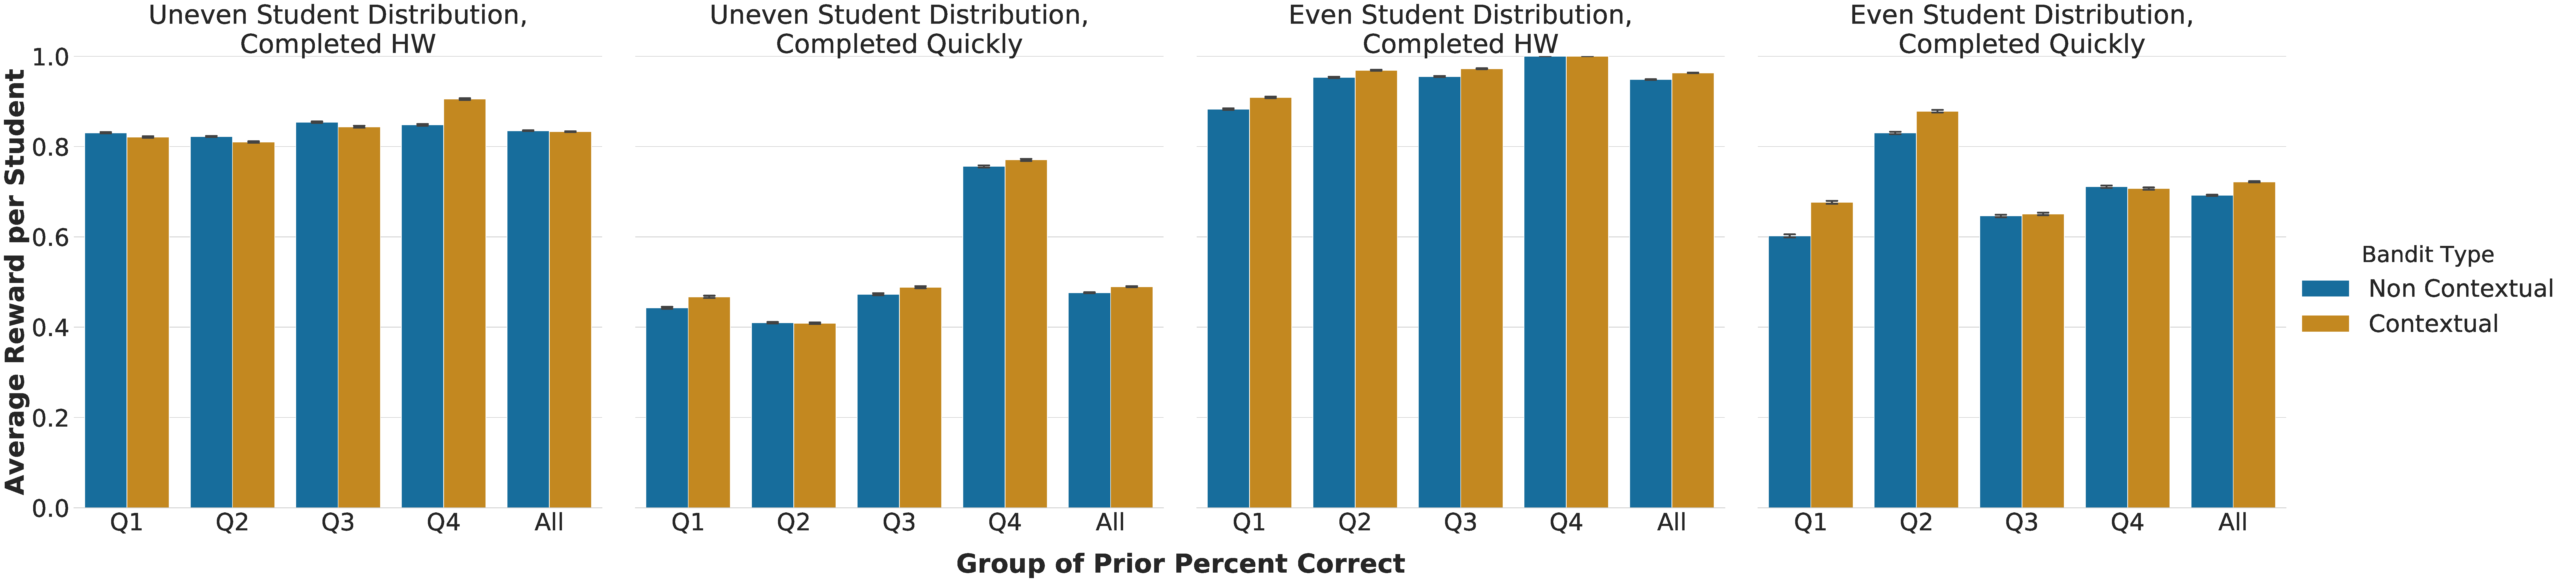
\includegraphics[width=\textwidth]{figs/RealWorld_AvgReward.pdf}
%     \caption{Average reward per student across the four quartiles of prior percent correct (Q1--Q4) and overall for the two bandit types. The bar graphs for the four simulation scenarios are generated by simulating classrooms at their original size (Table~\ref{table:realworldSimSetups}) over 1000 trials. Error bars represent 1 standard error.}
%     \label{fig:realworldReward}
% \end{figure*}

\begin{figure*}[t]
    \centering
    \includegraphics[width=\textwidth]{figs/RealWorld_SwarmHybridLabeled.pdf}
    \caption{Swarm plots for the proportion of optimal actions for the two bandit types for each quartile of prior percent correct and their averages. Each point represents results from each of the 1000 trials per experiment and the solid black lines indicate the means of each swarm plots. Points for Q4 of Even Student Distribution, Completed HW are clustered at 1.0 because both actions are optimal. The extra information learned by the contextual bandit improves performance in most cases but the bimodality for some quartiles demonstrates the associated systematic risks.}
    \label{fig:realworldDistribution}
\end{figure*}

For step (2), we simulate a MAB algorithm's performance by repeatedly sampling students from the experiment. Within each trial, we fix the number of timesteps to the total number of students in the original experiment. At each timestep, a random student is sampled, and the algorithm then selects a condition for that student.
% ; for the contextual MAB algorithm, the condition is dependent upon the student's prior percent correct.
To compute the outcome, we sample from all outcomes for students in the experiment who were in the same quartile for prior percent correct and who experienced the same chosen condition. Each trial thus represents an experiment of the same size as the original, with the students drawn with replacement from the experimental data. We randomized each of the 1000 trials, though for each trial, we use the same student ordering for both types of MAB algorithms.

In our case studies, we focus on one problem set (\#293151) where students are unevenly distributed across quartiles, with more lower-performing students (Q1), and one problem set (\#263057) in which students are more evenly distributed across quartiles (see Table~\ref{table:realworldSimSetups}).  
With the two different outcome measures, this resulted in four simulation scenarios.
We chose these problem sets because they had student outcomes that varied based on both condition and student quartile (see Figure~\ref{fig:realworldParameters}).
%, for the problem set where students were unevely distributed across quartiles, the highest performers (Q4) were helped more by the control condition than the experimental condition, while the opposite was true for the remaining students (Q1-Q3).  For the problem set with a more even distribution of students, the lowest performers (Q1) were 


\subsection{Results}

In all four settings, at least one quartile of students (out of Q1--Q4) was helped by the contextual MAB algorithm, and in three of the four settings, average outcomes across all students were improved by personalization. 


\textbf{Uneven Student Distribution, Completed HW:} As shown in Figure~\ref{fig:realworldDistribution}a, in this scenario, students in Q4 were much more likely to experience their optimal condition with a contextual MAB algorithm. This occurs because the condition that is best for the average student is the one that is worse for Q4: the non-contextual MAB thus optimizes in a way that has a systematic, negative outcome for Q4 students. Conversely, the contextual MAB algorithm does not do as well as the non-contextual algorithm for students in Q1--Q3 because of the extra exploration needed to learn about more variables that are not necessary to help these students. Overall, this means that the contextual MAB algorithm had a slightly lower rate of choosing the optimal action than the non-contextual MAB. However, the difference is relatively small, and is even smaller in terms of average reward: reward is reduced by less than $0.01$ overall, while is increased for Q4 students by about $0.06$. In this experiment, reward rates are high in general (greater than $70\%$ for all conditions and quartiles). Thus with 320 students, small differences in condition assignment often are not reflected in large differences in outcomes. Q1--Q3 students have very similar outcomes across the two methods of condition assignment; Q4 has the greatest difference in success for one condition versus another, and thus the large increase in optimal condition assignment for these students does boost the average outcomes. 

\textbf{Uneven Student Distribution, Completed Quickly:} Using the Completed Quickly outcome measure with the same students, students in all quartiles were more likely to be assigned to the optimal condition when the contextual MAB algorithm was used (Figure~\ref{fig:realworldDistribution}b). This pattern occurs because the overall probability of a positive outcome is very similar across the two conditions when student quartiles are ignored (shown by \textit{All} in Figure~\ref{fig:realworldParameters}b), making it difficult for the non-contextual bandit to learn that the experimental condition is better on average. In contrast, the differences between conditions are large for all quartiles except Q2. Thus, the information from the student quartiles makes the problem easier for the contextual MAB algorithm, though the relatively small difference between conditions for Q2 results in the lowest overall proportion of optimal action choices. This simulation thus importantly shows a scenario that was not explored in the prior simulations, in which knowing about extra information increases the number of  parameters to learn but makes learning about each of those individual parameters easier.

\textbf{Even Student Distribution, Completed HW:} For this scenario, there were again very high reward probabilities across all conditions, and a relatively small overall difference between conditions but larger differences between conditions for three of the four quartiles. The results from the previous simulation were mirrored here: all groups with some reward rates of less than $100\%$ were aided by the contextual MAB algorithm.

\textbf{Even Student Distribution, Completed Quickly:} Finally, using the Completed Quickly outcome measure for this second set of students, the results were still largely in favor of the contextual MAB algorithm. As the experimental condition is better on average, students in Q1 experience a large positive impact through personalization because the control condition is uniquely better for them. Q2 and Q3 also experience positive impacts, with the impact on Q2 students being larger because the difference between the two conditions is larger, which speeds learning for the contextual bandit. Conversely, Q4 students experience slightly less positive outcomes under the contextual MAB algorithm because the small difference between conditions slows learning; in comparison, the contextual MAB algorithm is more beneficial for Q4 students since the overall difference between conditions across all students is larger than the difference for Q4 students only. 

% in comparison, the overall difference across all students is larger between conditions than the difference only for Q4 students, so the non-contextual MAB algorithm uses this information and is thus more beneficial for Q4 students than the contextual MAB algorithm.

\textbf{Variability in real-world scenarios:} Variability across trials in these scenarios showed the same trend as in the previous simulations: the non-contextual MAB algorithm typically has slightly more variation around the mean of the distribution, but only the contextual MAB algorithm shows bimodality, with some trials showing very poor performance for at least one of the groups (Figure~\ref{fig:realworldDistribution}). 




















\begin{comment} We first modeled problem set 293151 with a completion reward scheme, under which students from quartiles 1--3 of Prior Percent Correct performed better under condition E, while students from quartile 4 performed better under condition C (see Table~\ref{table:observedParamsP293151}). As this was an example of group-dependent policy, we hypothesized that students from quartile 4, as the minority, would receive considerably more reward from the use of a contextual MAB compared to a non-contextual MAB, while the other groups would see slightly diminished reward, similar to the group dependent policy simulation shown above.

\begin{table}[h]
\label{table:observedParamsP293151}
\centering
\begin{tabular}{cc||c|c|c|c}
                           &   & \multicolumn{4}{c}{Accuracy Quartile}      \\
                           &   & $Q_1$  & $Q_2$  & $Q_3$  & $Q_4$  \\\hline\hline
\multirow{2}{*}{Condition} & C & 0.72   & 0.73   & 0.71   & 0.95   \\\cline{2-6}
                           & E & 0.83   & 0.83   & 0.87   & 0.77    
\end{tabular}
\caption{Observed student probability of completion for problem set 293151.}
\end{table}

As shown in the Table~\ref{table:observedParamsP293151}, for 375 students, quartiles 1--3 did indeed see slightly diminished reward (-1.020243 for quartile 0; -1.037975 for 1; -0.292887 for 2); however, the gain in reward for quartile 3 was also considerably slight (+2.866426). While these results are not in direct conflict with those from the group dependent policy simulation shown above, the end result is that total classroom reward for this problem set was considerably lower with a contextual MAB than with a non-contextual MAB, despite the group dependent policy. We believe that this is because the minority group is quartile 4 and has high reward and low variance. Therefore, the contextual bandit is less likely to explore and optimize effectively for that minority group. We hypothesized that if the minority group is quartile 1 and has low reward, then the contextual bandit should be able to explore and optimize effectively. 

In order to test this hypothesis, we next modeled problem set 263057 with the same completion reward scheme, under which students from quartile 1 performed better under condition C while students from quartiles 2--3 performed better under condition E, with similarly high proportions of reward in all quartiles as seen in problem set 293151 (see Table~\ref{table:observedParamsP263057}). Students from quartile 4 performed equally under both conditions, and thus this set was not a perfect match for our archetype for group-dependent policy, and that, assuming the null hypothesis, we would expect to see less gain in reward for quartile 1 in this case than for quartile 4 for the prior.

\begin{table}[h]
\label{table:observedParamsP263057}
\centering
\begin{tabular}{cc||c|c|c|c}
                           &   & \multicolumn{4}{c}{Accuracy Quartile}      \\
                           &   & $Q_1$  & $Q_2$  & $Q_3$  & $Q_4$  \\\hline\hline
\multirow{2}{*}{Condition} & C & 0.95   & 0.85   & 0.86   & 1.00 \\
                           & E & 0.86   & 1.00   & 1.00   & 1.00    
\end{tabular}
\caption{Observed student probability of completion for problem set 263057.}
\end{table}

Table~\ref{table:observedParamsP263057} shows the results: as expected, for 129 students, we found that the contextual MAB received slightly diminished reward relative to the non-contextual MAB for quartiles 2--4 ({-#} for quartile 2; {-#} for 3; {-#} for 4), but considerably increased reward for quartile 1 ({+#}). These results indicate that high probabilities influence the effectiveness of MAB models due to two factors: first, less reward is available to gain relative to the least beneficial condition; second, lower variance increases the likelihood that the MAB (especially contextual) will exploit the non-optimal condition. {...}

Next, we moved to modeling with observed difficulty reward in order to more closely match the probabilities of reward we had assumed in the simulations. We again worked with problem set 263057 which, under this reward scheme, saw students from quartile 1 performing better under condition C and students from quartiles 2--4 performing better under condition E, each by a substantial margin (see Table below). We hypothesized, as with the first experiment, that we would see performance differences similar to those observed in those in the simulation section above

\begin{table}[]
\begin{tabular}{lllll}
  & 0    & 1    & 2    & 3    \\
C & 0.74 & 0.69 & 0.57 & 0.69 \\
E & 0.50 & 0.93 & 0.69 &0.72    
\end{tabular}
\end{table}

However, this experiment also exhibited behavior that we had not considered in the simulations: as shown in Table {Y}, not only did the minority group, quartile 1, see great gain with the contextual MAB over the non-contextual (+1.425619), but the majority, quartiles 2--4, also benefited considerably (+0.795122 for quartile 1; +0.039711 for 2; +0.050724 for 3). {...}

Lastly, we modeled problem set 241622 with an observed difficulty reward scheme. These parameters saw students from all quartiles performing better under condition {C/E}, though by differing margins (see Table {X}), thus following a group-independent policy, group dependent reward pattern. As such, we hypothesized that our earlier finding from {Simulation X.Z} should hold that whenever the policy is group-independent, regardless of whether a contextual model would be more accurate to the data, the non-contextual MAB will produce better rewards.

The results, shown in Table {Y}, indicate that this principle holds in a modeled experiment: all groups saw diminished reward from the contextual MAB relative to the non-contextual MAB. Consistent with our findings in {Simulation X.Z}, while  
\end{comment}







\section{Discussion}

Real-time adaptive algorithms can respond quickly to optimize experiences for individual students, and their expressivity for personalizing experiences increases with each additional type of student information they are given. In this paper, we have shown that this expressivity is worthwhile only when it is \textit{necessary}  for expressing the best policy to improve student outcomes. It is also especially helpful in cases where student characteristics are not uniformly distributed. In that case, an algorithm without the extra information may instead learn a policy that systematically optimizes for the majority but not for a minority group. However, when this expressivity is not necessary, it increases variability across students and also increases the time for identifying the correct policy, thus significantly decreasing the number of students assigned the best version of the technology and slightly decreasing their average outcomes. Despite this, the results based on the real-world experimental data clarify the potential benefits of personalization by demonstrating that having extra information about students can sometimes make learning easier, outweighing the negative impact of learning additional parameters.


There are several limitations to our results. First, we have focused only on discrete student features and discrete outcomes but continuous parameters are also common. For example, we might measure student scores rather than homework completion or model prior knowledge as an estimated ability parameter. If one wanted to extend these analyses to real-valued student features, one could easily incorporate them into the current modeling framework with versions of Thompson sampling for real-valued outcomes~\cite{agrawal2013thompson}, and there exist metrics from a large literature for assessing whether students are treated fairly (e.g.,~\cite{binns2018fairness}). Using real-valued parameters is unlikely to significantly impact trends in results, except that defining student groups for analyzing equitable outcomes is more difficult. Our results from our universal optimal action scenarios show that, with binary rewards, knowledge of the student features is not beneficial if it is unnecessary for expressing the best policy. However, these results may not translate to the real-valued rewards case, where the latent student features will add to the variability in the distributions observed by the non-contextual bandit, and exploring these scenarios is an important step for future work. 
%However,  In contrast to binary outcomes, it is possible that there are cases with real-valued outcomes where knowledge of the student features is beneficial even if that knowledge is unnecessary to express the best policy. In the real-valued case, the latent student features will add to the variability in the distributions observed by the non-contextual bandit, and exploring these universal optimal action scenarios is an important step for future work. 
A second limitation is that our simulations comprise only a single student feature that influences the outcome, though in actual deployments multiple features may influence the best policy. Still, we believe that our results can guide system designers when thinking about such scenarios, especially in weighing the costs and benefits of including each possible variable.

%The real-world scenarios demonstrate that the MAB algorithms' achieve 

% - How different are rewards for MAB algortihms in real word versus a 50-50 split? 
% - How close are the MAB results to the best arm?
% - Why should we be concerned anyway? (variance, systematic differential treatment)
The results from the real-world scenarios highlight the potential value of MAB algorithms for educational technologies. For almost all scenarios and groups, both types of MAB algorithms chose the optimal condition more often than if students had been assigned uniformly at random, and average rewards were in many cases very close to the optimal expected reward (i.e. if the optimal action had been chosen for all students). The absolute difference in rewards was relatively small between the two bandit types--at most $0.075$--and the contextual bandit achieved at worst 12\% less than the optimal expected reward for any student group. Yet the earlier simulations urge caution for incorporating student characteristics, due to (1) decreases in achieved outcomes when these characteristics are unnecessary, (2) increases in variability of performance, and (3) the systematically different treatment of students based on irrelevant characteristics. Thus, system designers should weigh the risk of not personalizing when the best policy for the minority differs from the majority with these side effects of personalization and ultimately strive to only include variables that past evidence suggests differentially impact outcomes.
% Since the impact on a minority group of failing to include the possibility of personalization is largest when the best policy for that group differs from the majority group, designers could weigh this risk more heavily, while still including only variables that past evidence suggests are differentially related to outcomes. Additionally, system designers must take into account the greater variability across student experiences that is introduced by contextual MAB algorithms, particularly the ethical issues raised by treating  students systematically differently based on irrelevant characteristics.

% as the rate at which the system chose an optimal action was above 50\% for almost all scenarios and groups

% Our results highlight the difference between optimal choices by a system and the stochastic student outcomes that arise from those choices. When differences between versions of a technology are small, even the best choices may not lead to large observed differences in student outcomes. This is clear in some of the real-world experiments we examined, where the vast majority of students completed their homework regardless of their condition assignment. 
% % Both contextual and non-contextual MAB algorithms performed well on the real-world data, and for only one experiment and one quartile of students was expected performance below that 
% In general, it is difficult to design multiple versions of an educational technology that are all \textit{a priori} reasonable and that lead to large differences in outcomes. 
% Yet, educational technology improvement is precisely the goal of many experiments in fields like artificial intelligence and education, and even incremental differences may in aggregate lead to better experiences for students.
% Thus, even though the average differences in outcomes across bandit types are relatively small, they should be a consideration for system designers. Since the impact on a minority group of failing to include the possibility of personalization is largest when the best policy for that group differs from the majority group, designers could weigh this risk more heavily, while still including only variables that past evidence suggests are differentially related to outcomes. Additionally, system designers must take into account the greater variability across student experiences that is introduced by contextual MAB algorithms, particularly the ethical issues raised by treating  students systematically differently based on irrelevant characteristics.

One could make a number of extensions of this work for using MAB algorithms to improve and personalize educational technologies. First, contextual MAB algorithms might mitigate issues of biases when different types of students interact with an educational technology and while all are most helped by the same version of the technology, their outcomes have different distributions. For example, struggling students may complete homework later, leading the MAB algorithm's early estimates to be non-representative of the broader population. Prior work has shown that this bias significantly worsens inference about the effectiveness of the technology as well as expected student outcomes~\cite{rafferty2019statistical}: the use of a contextual MAB algorithm could allow the system to adapt to such differences across students. Second, if the technology is used by a large number of students, the set of variables used by the contextual algorithm could be increased as more data are collected. Such a system might improve consistency across student outcomes, while still personalizing based on truly relevant features that are justified the sufficient information collected. The work in this paper both provides a starting point for considering what scenarios, algorithms, and metrics should be explored in future work, as well as guidance for system designers who would like to deploy MAB algorithms within their own technologies but are uncertain about which student characteristics, if any, to include for personalization.


% % Include something in here about possibility of partially sharing information across actions [ANR: What did I mean by that?]
% Topics to discuss:
% \begin{itemize}
%     \item Binary versus real-valued (Would this make a difference for the group-dependent reward scenarios?)
%     \item Rewards versus optimal actions - real-world impacts
%     \item Knowing about student characteristics could help mitivate differences in when different types of students participate (e.g., if students who are struggling tend to complete homework later).
% \end{itemize}


\pagebreak

\bibliographystyle{abbrv}
\bibliography{CompiledBib}


\balancecolumns
\end{document}
